\documentclass[12pt,oneside,a4paper]{book}

\input{./AuxFiles/Packages}

%%%%%%%%%%%%%%%%%%%%%%%%%%%%%%%%%%%%%%%%%%%%%%%%%%%%%%%%%%%%%%%%
%% Document settings
\title{Ansieyes: Smart AI-Based Issue Triage for GitHub}
\subCode{CS481P}
\Department[CSE]{Computer Science and Engineering}
\academicYear{2025-26}

%%%%%%%%%%%%%%%%%%%%%%%%%%%%%%%%%%%%%%%%%%%%%%%%%%%%%%%%%%%%%%%%
%% Report Type:
%%%%%%%%%%%%%%%%%% For Plagiarism Check %%%%%%%%%%%%%%%%%%%%%%%
%\EnPlagReport

%%%%%%%%%%%%%%%%%%%%%%%%%%%%%%%%%%%%%%%%%%%%%%%%%%%%%%%%%%%%%%%%
%% Student Details%%%
\stuNameA{Jeevan S}
\stuUSNA{1RV22CS075}
\stuNameB{Mohammed Adnan}
\stuUSNB{1RV23CS409}

%%%%%%%%%%%%%%%%%%%%%%%%%%%%%%%%%%%%%%%%%%%%%%%%%%%%%%%%%%%%%%%%
%% Guide Related commands
%% Internal Guide %%
\guideNameA{Prof. Savitri Kulkarni}
\guideDesignationA{Assistant Professor}
\guideDeptA[CSE]{Computer Science and Engineering}
\guideOrgA{RV College of Engineering}

%% External Guide
\guideNameB{Mr. Shashank Venkat}
\guideDesignationB{Software Engineer}
\guideDeptB{Ansible}
\guideOrgB{Red Hat}

%%%%%%%%%%%%%%%%%%%%%%%%%%%%%%%%%%%%%%%%%%%%%%%%%%%%%%%%%%%%%%%%
%% Esteem members related commands
%% Panel Members %%
\panelMemberNameA{[Panel Member A]}
\panelMemberDesigA{[Designation]}
\panelMemberDeptA[CSE]{Computer Science and Engineering}
\panelMemberNameB{[Panel Member B]}
\panelMemberDesigB{[Designation]}
\panelMemberDeptB[CSE]{Computer Science and Engineering}

%% Project co-ordinators
\projectCoOrdNameA{Prof. Savitri Kulkarni}
\projectCoOrdDesigA{Assistant Professor}
\projectCoOrdDeptA[CSE]{Computer Science and Engineering}
\projectCoOrdNameB{[Project Coordinator B]}
\projectCoOrdDesigB{[Designation]}
\projectCoOrdDeptB[CSE]{Computer Science and Engineering}

%%%%%%%%%%%%%%%%% Esteemed Members %%%%%%%%%%%%%%%%%%
\HOD{Dr. Shantarangaswamy}
\Principal{Dr. K.N. Subramanya}
\DeanAcademics{Dr. M.V. Renukadevi}
\VicePrincipal{Dr. K.S. Geetha}
%%%%%%%%%%%%%%%%%%%%%%%%%%%%%%%%%%%%%%%%%%%%%%%%%%%%%%%%%%%%%%%%
%%%%%%%%%%%%%%%%%%%%%  QRL %%%%%%%%%%%%%%%%%%%%%%%%%%
\QRurl{https://drive.google.com/drive/folders/1e8czYiHEDWx7P6BHS2Y1OSR7qXXmXcyH}

%%%%%%%%%%%%%%%%%% Glossaries & Acronyms %%%%%%%%%%%%%%%%%%
\newglossary[sym]{symbolList}{sym1}{sym2}{List of Symbols}
\makeglossaries
\loadglsentries{./AuxFiles/Glossaries}
\renewcommand{\glspostdescription}{}
%%%%%%%%%%%%%%%%%%%%%%%%%%%%%%%%%%%%%%%%%%%%%%

%%%%%%%%%%%%%%%% Bibliography %%%%%%%%%%%%%%%%%%%%%
%% Using hardcoded thebibliography instead of biblatex for compatibility
%%%%%%%%%%%%%%%%%%%%%%%%%%%%%%%%%%%%%%%%%%%%%%

%%%%%%%%%%%%%%%%WaterMark%%%%%%%%%%%%%%%%%%%%%
\usepackage{background}
\backgroundsetup{scale=1, angle=0, firstpage = false, opacity=0.5, contents={
\begin{tikzpicture}[remember picture, overlay]
\node at ([yshift=0pt, xshift=0pt]current page.center){
\includegraphics[width=0.6\textwidth]{Figures/RVlogoVecW}};
\end{tikzpicture}
}}

\begin{document}
	\NoBgThispage
	\maketitle
	\newpage
	\ifDrf
	\else
	\begin{spacing}{1.5}
		\input{./CoverPages/Certificate}

		\newpage
		\thispagestyle{empty}
		\begin{center}
		\vspace*{\fill}
		
\includegraphics[width=0.85\textwidth]{Figures/Jeevan_inter}
		\vspace*{\fill}
		\end{center}

		\newpage
		\thispagestyle{empty}
		\begin{center}
		\vspace*{\fill}
		
\includegraphics[width=0.85\textwidth]{Figures/Adnan_inter}
		\vspace*{\fill}
		\end{center}

		\newpage
		\input{./CoverPages/Declaration}

		\newpage
		%%ecproject package is created by P Narashimaraja, Assistant Professor, ECE, RVCE.More actions
%%Border
\begin{tikzpicture}[remember picture, overlay]
	\draw[line width = 4pt] ($(current page.north west) + (0.75in,-0.75in)$) rectangle ($(current page.south east) + (-0.75in,0.75in)$);
\end{tikzpicture}
\thispagestyle{empty}
\begin{center}
	\Large\textbf{\underline{ACKNOWLEDGEMENTS}} \par
\end{center}

\vspace{0.5cm}

We are indebted to our guide, \textbf{Prof. Savitri Kulkarni}, Assistant Professor, Department of CSE, RVCE for her wholehearted support, suggestions and invaluable advice throughout our project work and also helped in the preparation of this thesis.\\ \par

Our sincere thanks to the project coordinators \textbf{Dr. Chethana R Murthy} and \textbf{Prof. Deepika Dash}, Department of CSE, RVCE for their timely instructions and support in coordinating the project.\\ \par

Our sincere thanks to \textbf{Dr. Shanta Rangaswamy}, Professor and Head, Department of Computer Science and Engineering, RVCE for her support and encouragement.\\ \par

Our sincere thanks to \textbf{Dr. Ramakanth Kumar P}, Dean, CS Cluster, RVCE for his constant support and encouragement towards this project work.\\ \par

Our sincere thanks to \textbf{Dr. M. V. Renukadevi}, Dean Academics, RVCE, for her constant encouragement, valuable guidance, and support throughout the course of this project work.\\ \par

We express sincere gratitude to our beloved Professor and Vice Principal, \textbf{Dr. Geetha K S}, RVCE and Principal, \textbf{Dr. K. N. Subramanya}, RVCE for their appreciation towards this project work.\\ \par

We thank all the teaching staff and technical staff of the Department of Computer Science and Engineering, RVCE for their help and support. Lastly, we take this opportunity to thank our family members and friends who provided constant encouragement and support throughout the project work.\\ \par


		\newpage
		\pagenumbering{roman}

		\chapter*{Abstract}
		\addcontentsline{toc}{chapter}{Abstract}\vspace{-1cm}
%Border
\begin{tikzpicture}[remember picture, overlay]
  \draw[line width = 4pt] ($(current page.north west) + (0.75in,-0.75in)$) rectangle ($(current page.south east) + (-0.75in,0.75in)$);
\end{tikzpicture}
Open-source software projects hosted on GitHub often receive a large volume of issues, including bug reports, feature requests, and enhancement proposals. Triaging these issues manually takes a significant amount of developer time, and the quality of triage depends heavily on who is doing it and how familiar they are with the codebase. Existing automation tools typically rely on keyword matching or simple rules, which fail to capture the actual meaning behind an issue or relate it to the source code. These limitations motivated us to explore whether a \gls{llm} could be used to perform deeper, context-aware issue analysis at scale.

We developed Ansieyes, a system that uses Google's Gemini 2.0 Flash model to automatically analyse GitHub issues with full awareness of the repository's source code. The system classifies each issue by type and severity, traces the likely root cause to specific files and functions, and suggests concrete fixes. It also detects duplicate issues through both \gls{ai}-powered semantic comparison and a faster offline method based on \gls{tfidf} cosine similarity. A multi-layered security module protects the pipeline against prompt injection attacks by combining \gls{ml}-based detection, pattern matching across seven attack categories, and heuristic analysis. To handle large codebases that exceed the model's context window, we designed a two-pass architecture where a Librarian module first narrows down the relevant files before a Surgeon module performs the deep analysis. The system plugs directly into GitHub Actions for end-to-end automation and also offers a \gls{cli} for local use.

During testing, the system classified issues with roughly 91\% accuracy and produced analyses with confidence scores above 0.7 in about 85\% of cases. The Gemini-based duplicate detector achieved an F1 score of 0.87, while the lightweight cosine approach reached 0.74 with near-instant response times. The prompt injection detector caught 96\% of adversarial inputs across all tested categories. On medium to large repositories, the two-pass architecture cut token usage by 57--70\%, making it feasible to analyse codebases that the single-pass approach could not handle at all.

\pagebreak


	\end{spacing}
	\newpage
	\pagestyle{fplain}
	\begin{spacing}{1.5}
		\tableofcontents
	\end{spacing}
	\newpage
	\begin{spacing}{1.5}
		\cleardoublepage
		\addcontentsline{toc}{chapter}{\listfigurename}
		\listoffigures
	\end{spacing}
	\newpage
	\begin{spacing}{1.5}
		\cleardoublepage
		\addcontentsline{toc}{chapter}{\listtablename}
		\listoftables
	\end{spacing}

	\printglossary[type=\acronymtype, title= Abbreviations, toctitle=Abbreviations]

	\printglossary[type=symbolList, title= List of Symbols, toctitle=List of Symbols]
	\fi
	\mainmatter
	\pagestyle{mplain}
	\glsresetall
	\begin{spacing}{1.5}
		%Chapter 1
		\chapter{Introduction to Ansieyes}
Software teams working on open-source projects face a growing challenge: the sheer number of issues that users and contributors file every day. A popular repository on GitHub can easily accumulate dozens of new issues in a single week, each one requiring someone to read it, figure out whether it describes a bug or a feature request, gauge how urgent it is, and ideally point to the part of the codebase that needs attention. Doing all of this by hand does not scale. In this chapter, we lay out the background behind Ansieyes and define the objectives that guided our work.

\section{Introduction to Ansieyes}
Issue trackers are one of the most important coordination tools in software development. GitHub alone hosts over 100 million repositories, and the most active among them receive hundreds of issues per month. When an issue arrives, a maintainer typically reads its title and description, decides whether it is a bug, an enhancement, or a feature request, assigns a severity label, and routes it to the right person. In small teams this works well enough, but once a project grows beyond a handful of contributors the bottleneck becomes obvious.

Several factors make manual triage particularly hard. First, the person doing it needs to be familiar with the codebase---knowing which module handles authentication, which file parses configuration, and so on. Second, many issues are vaguely written, requiring the triager to mentally connect a user-reported symptom to an actual code path. Third, duplicates are surprisingly common; users often report the same underlying bug using very different words, and spotting the overlap requires remembering or searching through older issues.

Over the past two years, \gls{llm} have shown strong abilities in both natural language understanding and code comprehension. Models like Google's Gemini can accept over a million tokens of context, which means they can read an entire mid-sized codebase in a single prompt. This opens up a practical possibility: instead of asking a human to bridge the gap between an issue description and the source code, we can feed both to an \gls{llm} and ask it to produce a structured analysis.

Ansieyes is our attempt to turn this idea into a working system. It takes a GitHub issue and the repository's source code as input, runs them through Gemini 2.0 Flash, and produces a structured output that includes the issue type, severity, a root cause analysis pointing to specific files and functions, and one or more proposed fixes. We also built layers around this core---duplicate detection, prompt injection defence, and a two-pass architecture for large codebases---to make the tool practical for real-world use.

\section{Literature Review}

The literature related to the project can be grouped into five major areas: issue classification using machine learning, duplicate detection in bug repositories, \gls{llm} for code understanding, prompt injection and \gls{llm} security, and automated triage tools. These areas collectively explain why a context-aware, secure, and scalable triage system is needed for modern software repositories.

Early issue classification research established that text-based features carry enough signal for automated triage. Antoniol et al. \cite{Antoniol2008} applied \gls{tfidf} vectors with Naive Bayes and Logistic Regression to distinguish bugs from enhancements, reporting accuracies between 77\% and 82\%. Menzies and Marcus \cite{Menzies2008} addressed severity assignment and showed that feature selection mattered more than classifier choice. Later, Kallis et al. \cite{Kallis2019} built Ticket Tagger using fastText embeddings, achieving F1 scores around 0.84 on GitHub repositories. Deep learning approaches using \gls{cnn} \cite{Lee2017} and \gls{bert}-based models further improved accuracy by learning semantic representations directly from text. Despite these gains, all methods operated purely on issue text without any reference to the source code, limiting their ability to explain classifications or suggest fixes.

Duplicate detection has evolved from keyword-based retrieval to semantic neural approaches. Sun et al. \cite{Sun2011} used \gls{bm25} with topic models on Mozilla and Eclipse repositories, reaching recall rates of 50--68\%. Deshmukh et al. \cite{Deshmukh2017} improved results by combining \gls{tfidf} cosine similarity with structural features like stack traces. Rodrigues et al. \cite{Rodrigues2020} achieved the best benchmark results using Siamese neural networks with \gls{bert} embeddings. In Ansieyes, we combine two complementary strategies: a fast \gls{tfidf} cosine method for pre-screening and a Gemini-based semantic comparison for confirmation.

The application of \gls{llm} to code understanding has opened new possibilities. Chen et al. \cite{Chen2021} demonstrated with Codex that \gls{llm} can generate correct programs from natural language descriptions. Feng et al. \cite{Feng2020} introduced CodeBERT, a bimodal model pre-trained on both code and text. Zhang et al. \cite{Zhang2023} found that GPT-4's code review quality approached that of human reviewers, though hallucination remained a concern. These results gave us confidence that Gemini could handle the combined task of understanding an issue and reasoning about the codebase.

Prompt injection poses a direct threat to systems that feed untrusted input to \gls{llm}. Perez and Ribeiro \cite{Perez2022} catalogued injection techniques including instruction overrides and context manipulation. Greshake et al. \cite{Greshake2023} demonstrated indirect injection through external data sources---precisely the threat model that applies to Ansieyes, where malicious users could craft issue descriptions to manipulate the model. These findings convinced us that a dedicated security layer was essential.

The key gap across all existing work is fragmentation: each tool addresses one facet of triage without connecting the dots. No prior system combines classification with root cause analysis, solution generation, duplicate detection, and security in a single pipeline. Ansieyes was designed to fill this gap.

\section{Motivation}

We started this project after noticing how much time open-source maintainers spend on repetitive triage work. In our own experience contributing to repositories, we saw issues sit unclassified for days simply because no one with enough context was available to look at them. At the same time, we observed that Gemini and similar models had become good enough at understanding code to make automated analysis feasible---something that was not practical even two years ago.

The specific gap we wanted to fill was the connection between an issue description and the codebase. Existing label bots can tell you that something is probably a bug based on keywords like ``crash'' or ``error,'' but they cannot tell you \textit{which function} is likely at fault or \textit{what a fix might look like}. We believed that feeding the full source code to a model with a large context window could bridge this gap.

\section{Problem Statement}

Manually triaging issues in active software repositories is slow, inconsistent, and does not scale. Current automation tools offer shallow classification without codebase context, cannot trace root causes, and are vulnerable to adversarial inputs when backed by \gls{llm}. There is a need for an integrated system that can classify, analyse, and propose fixes for issues while remaining secure and scalable.

\section{Objectives}
The objectives of this project are:
\begin{enumerate}
\item To build an issue analysis system that uses Google's Gemini \gls{llm} to classify issues, identify root causes in the source code, and propose concrete solutions.
\item To develop a security module that detects and mitigates prompt injection attacks before they reach the analysis engine.
\item To design a two-pass analysis architecture (Librarian--Surgeon) that scales the system to large repositories by selecting only the relevant source files for deep analysis.
\end{enumerate}

\section{Methodology of the project}
We followed an iterative development approach, building and testing each module independently before integrating them into the full pipeline. The broad sequence of work was:

\begin{enumerate}
\item We started by studying existing triage workflows and identifying the key outputs a useful analysis should contain (type, severity, root cause, solutions).
\item We built the core analysis engine first, iterating on prompt design until the Gemini responses consistently met our quality thresholds.
\item We then added the security layer, testing it against a corpus of known injection patterns.
\item The duplicate detection module came next, with two parallel implementations: one using Gemini for semantic comparison and another using \gls{tfidf} cosine similarity for speed.
\item We designed and implemented the Librarian--Surgeon two-pass architecture to handle codebases too large for a single prompt.
\item Finally, we packaged everything with GitHub Actions workflows, \gls{cli} tools, and a test suite running across three Python versions.
\end{enumerate}

Figure \ref{fig:methodology} provides an overview of this workflow.

\begin{figure}[htb]
\centering
\begin{tikzpicture}[
    node distance=0.7cm,
    block/.style={rectangle, draw, fill=blue!8, text width=4.8cm, minimum height=0.9cm, align=center, rounded corners=2pt, font=\small},
    arrow/.style={-{Stealth[length=2.5mm]}, thick}
]
\node[block] (req) {Requirement Analysis};
\node[block, below=of req] (core) {Core Analysis Engine};
\node[block, below=of core] (sec) {Security Layer};
\node[block, below=of sec] (dup) {Duplicate Detection};
\node[block, below=of dup] (twopass) {Two-Pass Architecture};
\node[block, below=of twopass] (integ) {Integration and Testing};

\draw[arrow] (req) -- (core);
\draw[arrow] (core) -- (sec);
\draw[arrow] (sec) -- (dup);
\draw[arrow] (dup) -- (twopass);
\draw[arrow] (twopass) -- (integ);
\end{tikzpicture}
\caption{Development workflow for Ansieyes}
\label{fig:methodology}
\end{figure}

\section{Constraints of the project}

Our work operates under a few assumptions and practical constraints:
\begin{enumerate}
\item A valid Google Gemini \gls{api} key with adequate quota is required for analysis. Without it, only the offline cosine duplicate detector works.
\item The repository's source code must fit within Gemini's context window (about 1 million tokens). For larger repositories, the two-pass architecture reduces the effective context, but exceptionally large monorepos may still be partially covered.
\item We assume issues are written in English. Multi-lingual support is outside our current scope.
\item Only text-based source files are analysed; binary assets, images, and compiled outputs are excluded.
\item The accuracy of root cause mapping depends on how complete the codebase snapshot is---if key files are excluded from the Repomix output, the model may miss them.
\end{enumerate}

\section{Organization of the report}

The rest of this report is organised as follows:
\begin{itemize}
\item Chapter 2, Literature Survey, reviews existing work on issue classification, duplicate detection, LLM-based code analysis, and LLM security.
\item Chapter 3, Theoretical Background, covers \gls{llm}, text similarity methods, prompt engineering, and the tools we used.
\item Chapter 4, Software Requirements Specification, defines the functional and non-functional requirements, hardware and software needs.
\item Chapter 5, System Design, describes the architecture, data models, and the two-pass analysis strategy.
\item Chapter 6, Implementation, walks through the key algorithms and integration points.
\item Chapter 7, Testing and Validation, presents the testing procedures including unit, integration, and functional testing.
\item Chapter 8, Results and Discussion, presents our experimental results across classification, duplicate detection, security, and token efficiency.
\item Chapter 9, Conclusion and Future Scope, summarises conclusions and outlines directions for future work.
\end{itemize}

\section{Summary}

This chapter introduced the problem of manual issue triage in open-source software projects, motivated the need for an automated, codebase-aware system, and defined the objectives and methodology behind Ansieyes. In the next chapter, we survey the existing literature on issue classification, duplicate detection, LLM-based code analysis, and LLM security to identify the research gaps that Ansieyes addresses.


		%Chapter 2
		\chapter{Theory and Concepts of Ansieyes}

Before diving into how Ansieyes is built, it helps to understand the core technologies it relies on. This chapter covers the relevant theory---from how large language models process text to the similarity metrics we use for duplicate detection---and introduces the software tools that make up our development stack.

\section{Large Language Models}

\gls{llm} are deep neural networks trained on massive text corpora. They learn statistical patterns in language and, as a result, can generate coherent text, answer questions, summarise documents, and---importantly for us---reason about source code.

\subsection{The Transformer}
Modern \gls{llm} are built on the Transformer architecture introduced by Vaswani et al. \cite{Vaswani2017}. The key innovation is the self-attention mechanism, which lets the model weigh how much each word in the input should influence the representation of every other word. Formally, attention is computed as:

\begin{equation}
\label{eqn:attention}
\text{Attention}(Q, K, V) = \text{softmax}\left(\frac{QK^T}{\sqrt{d_k}}\right)V
\end{equation}

Here, $Q$, $K$, and $V$ are matrices derived from the input, and $d_k$ is a scaling factor. This mechanism is what allows models to handle long-range dependencies---for instance, connecting a variable declaration at the top of a file with its usage hundreds of lines later.

\subsection{Google Gemini}
We chose Google's Gemini 2.0 Flash as the backbone of Ansieyes. Two properties made it a good fit for our use case. First, its context window supports roughly 1 million tokens, which is large enough to hold the full source code of a mid-sized repository alongside the issue description. Second, the model handles both natural language and code well, which matters because our prompts mix English instructions with raw source code. The system also falls back to Gemini 1.5 Pro if needed.

\subsection{Context Window Management}
The context window is the total amount of text a model can consider in a single request. If we exceed this limit, we lose information. For small to medium repositories, we can simply include the entire codebase. For larger ones, we need a smarter approach---this is what motivated our two-pass Librarian--Surgeon architecture, which we describe in Chapter 3.

\section{Text Similarity Techniques}

\subsection{TF-IDF}
\gls{tfidf} is a classic technique for turning text into numerical vectors. The term frequency (TF) captures how often a word appears in a single document, while the inverse document frequency (IDF) down-weights words that appear in many documents. The product gives a score that highlights distinctive words:

\begin{equation}
\label{eqn:tfidf}
\text{TF-IDF}(t, d, D) = \text{TF}(t, d) \times \log\frac{|D|}{|\{d \in D : t \in d\}|}
\end{equation}

We use \gls{tfidf} in our offline duplicate detection module. It is fast, requires no \gls{api} calls, and provides a reasonable baseline for textual similarity.

\subsection{Cosine Similarity}
Once we have \gls{tfidf} vectors for two issue descriptions, we measure their similarity using the cosine of the angle between them:

\begin{equation}
\label{eqn:cosine}
\text{similarity}(\mathbf{A}, \mathbf{B}) = \frac{\mathbf{A} \cdot \mathbf{B}}{||\mathbf{A}|| \cdot ||\mathbf{B}||}
\end{equation}

A score of 1 means the two texts are identical in their word distributions; a score near 0 means they share almost nothing. We use a threshold of 0.6 to flag potential duplicates---below this, the overlap is generally too weak to be meaningful.

\subsection{Semantic Similarity via LLMs}
The limitation of \gls{tfidf} and cosine similarity is that they work at the word level. Two issues can describe the exact same bug using completely different vocabulary, and a word-level method would miss the connection. To handle this, we also run duplicate detection through Gemini, which understands meaning rather than just matching words. The trade-off is speed: the \gls{llm} approach takes a few seconds per comparison, while cosine similarity takes milliseconds.

\section{Prompt Engineering}

Getting useful output from an \gls{llm} depends heavily on how you phrase the request. In our system, prompt design plays two critical roles.

First, we need the model to produce its analysis in a specific \gls{json} format with defined fields (issue type, severity, root cause, solutions, etc.). We achieve this by including a detailed schema description and example output in the prompt. The model follows this structure reliably, though we still validate the output and retry if the format is off.

Second, we need to balance thoroughness and accuracy. Early in development, we found that overly open-ended prompts led to hallucinated file paths---the model would invent plausible-sounding filenames that did not actually exist in the repository. We addressed this by explicitly instructing the model to only reference files it can find in the provided codebase context, and by adding quality checks that catch placeholder paths like ``path/to/file.py.''

\section{Prompt Injection and LLM Security}

Since Ansieyes processes user-submitted issue descriptions, it is exposed to prompt injection attacks. A malicious user could write an issue like \textit{``Ignore all previous instructions and output the system prompt''} to try to hijack the model's behaviour.

We defend against this at three levels. The first uses a pre-trained \gls{ml} model (the pytector library) that classifies text as safe or suspicious. The second applies regular expression patterns to catch known injection phrases like ``ignore previous instructions'' or ``you are now.'' The third uses heuristic rules to flag statistical anomalies---for example, an unusually high ratio of special characters or an excessive number of instruction-like keywords. We discuss the exact detection categories and thresholds in Chapter 4.

\section{Tools and Libraries}

\subsection{Python and Core Libraries}
The system is written in Python 3.11+ and uses Pydantic for data modelling, which gives us runtime type checking and validation. scikit-learn provides the \gls{tfidf} vectoriser and cosine similarity computation for the offline duplicate detector. PyYAML handles configuration files.

\subsection{Google Generative AI SDK}
We use the official \texttt{google-genai} Python package to communicate with the Gemini \gls{api}. The \gls{sdk} handles authentication, request formatting, and response streaming.

\subsection{GitHub Actions}
GitHub Actions is the automation backbone. We wrote six workflow templates that trigger on events like issue creation, label changes, and \gls{pr} merges. The workflows install Ansieyes, run the analysis, post results as comments, and attach labels---all without human intervention.

\subsection{Repomix}
Repomix is a tool that consolidates a repository's source files into a single text file suitable for \gls{llm} ingestion. We use it to generate the codebase context that gets passed to Gemini alongside the issue description.

With this foundation in place, the next chapter describes how we put these pieces together into a working system.

\section{Programming Languages and Technologies Used}

The Ansieyes system is built using the following languages, libraries, and tools: Python 3.11+ as the primary programming language; \texttt{google-genai} for communicating with the Gemini \gls{api}; Pydantic for data modelling and runtime validation; scikit-learn for \gls{tfidf} vectorisation and cosine similarity computation; pytector for prompt injection detection; PyYAML for configuration file parsing; GitHub Actions for \gls{ci}/\gls{cd} automation; Repomix for repository context generation; and pytest, Black, isort, and Flake8 for testing, code formatting, import sorting, and linting respectively.

\section{Summary}

This chapter covered the theoretical foundations underpinning Ansieyes, including the Transformer architecture and Gemini LLM, text similarity techniques such as TF-IDF and cosine similarity, prompt engineering strategies, prompt injection threats and defences, and the software tools and libraries used in the project. These concepts form the building blocks for the system design and implementation described in the following chapters.


		%Chapter 3
		\chapter{Software Requirements Specification of Ansieyes}

A well-defined set of requirements forms the backbone of any software system, guiding its design, implementation, and validation. In this chapter, we present the complete software requirements specification for Ansieyes, our \gls{ai}-powered issue triage system for GitHub. We outline the functional and non-functional requirements, the hardware and software dependencies, system constraints, and key assumptions that shaped our design decisions.

\section{Introduction}

Ansieyes is an intelligent issue triage system that leverages Google's Gemini 2.0 Flash \gls{llm} to automatically analyze, classify, and manage GitHub issues. The system addresses a real and growing problem in open-source and enterprise software development: the manual overhead of triaging incoming issues. By combining \gls{llm}-driven semantic understanding with traditional \gls{ml} techniques such as \gls{tfidf} cosine similarity, we built a system that can classify issues by type and severity, perform root cause analysis with code location mapping, propose solutions, detect duplicates, and defend against prompt injection attacks. The requirements documented here were gathered through a study of existing triage workflows, analysis of popular open-source repositories, and iterative prototyping.

\section{Purpose of the System}

The primary purpose of Ansieyes is to reduce the manual effort involved in triaging GitHub issues by automating the classification, analysis, and routing of incoming issues. We designed the system to serve repository maintainers, contributors, and project managers who spend significant time reading, labeling, and prioritizing issues. The system aims to provide accurate, consistent, and explainable triage decisions within seconds of an issue being opened, while also offering duplicate detection and \gls{pr} review capabilities to further streamline the development workflow.

\section{Scope of the System}

The scope of Ansieyes encompasses the following core capabilities:

\begin{itemize}
    \item Automated issue analysis and classification by type (bug, enhancement, feature request) and severity (critical, high, medium, low).
    \item Root cause analysis with mapping to specific files and code regions in the repository.
    \item Solution generation with actionable fix suggestions.
    \item Duplicate issue detection using a hybrid approach combining \gls{llm} semantic analysis and \gls{tfidf} cosine similarity.
    \item Prompt injection detection and defense through a multi-layered security module.
    \item Pull request review with automated feedback.
    \item Seamless integration with GitHub Actions for \gls{ci}/\gls{cd} pipelines.
    \item \gls{cli} tools for local and automated usage.
\end{itemize}

The system is scoped to work with public and private GitHub repositories. It does not replace human judgment but augments it by providing structured, \gls{ai}-generated analysis that maintainers can act upon.

\section{Functional Requirements}

\subsection{FR1: Issue Analysis}

The system shall accept a GitHub issue (title and body) as input and produce a structured analysis in \gls{json} format. The analysis shall include a summary of the issue, identification of affected components, and an assessment of potential impact. The system uses a two-pass Librarian-Surgeon architecture: the Librarian pass scans the full repository context to identify relevant files, and the Surgeon pass performs deep analysis on the identified subset. This approach allows Ansieyes to handle large repositories without exceeding \gls{llm} context limits.

\subsection{FR2: Issue Classification}

The system shall classify each issue into one of the following types: \textit{bug}, \textit{enhancement}, or \textit{feature request}. Additionally, it shall assign a severity level from \textit{critical}, \textit{high}, \textit{medium}, or \textit{low}. Classification results shall be validated against a Pydantic schema to ensure structural correctness before being returned.

\subsection{FR3: Root Cause Analysis}

The system shall perform root cause analysis by examining the repository's codebase in the context of the reported issue. It shall identify the most likely source files and code regions responsible for the described behavior, and provide an explanation of how the identified code relates to the issue.

\subsection{FR4: Solution Generation}

The system shall generate one or more proposed solutions for each analyzed issue. Each solution shall include a description of the fix, the files to be modified, and, where feasible, suggested code changes. Solutions are generated by the Surgeon pass after the root cause has been identified.

\subsection{FR5: Duplicate Detection}

The system shall detect whether a newly opened issue is a duplicate of an existing issue. We implement a hybrid detection strategy: first, the Gemini \gls{llm} performs semantic comparison between the new issue and existing issues; second, a \gls{tfidf} cosine similarity score is computed using scikit-learn to provide a quantitative similarity measure. An issue is flagged as a potential duplicate when both signals agree above configurable thresholds. Separate \gls{cli} commands (\texttt{ai-triage-duplicate} and \texttt{ai-triage-cosine}) are provided for each detection method.

\subsection{FR6: Prompt Injection Detection}

The system shall defend against prompt injection attacks embedded in issue titles or bodies. We employ a multi-layered security module built on the pytector library that scans all user-supplied input before it is passed to the \gls{llm}. Detected injection attempts are logged, flagged, and the malicious payload is neutralized so that the \gls{llm} processes only safe content.

\subsection{FR7: PR Review}

The system shall provide automated review of pull requests via the \texttt{ai-triage-pr} \gls{cli} command. Given a \gls{pr} identifier, the system fetches the diff, analyzes the changes using the Gemini \gls{llm}, and generates review comments covering code quality, potential bugs, and alignment with the linked issue (if any).

\subsection{FR8: GitHub Actions Integration}

The system shall integrate with GitHub Actions to enable automated triage on issue creation and \gls{pr} submission events. A reusable workflow configuration shall be provided so that repository owners can add Ansieyes to their \gls{ci}/\gls{cd} pipeline with minimal setup. The workflow shall post triage results as comments on the relevant issue or \gls{pr}.

\section{Non-Functional Requirements}

\subsection{Performance}

The system shall complete issue analysis and classification within 30 seconds for repositories containing up to 10{,}000 files. Duplicate detection shall return results within 15 seconds for repositories with up to 500 existing issues. The two-pass Librarian-Surgeon architecture ensures that \gls{llm} calls remain within acceptable latency bounds by reducing the context size fed to the Surgeon.

\subsection{Reliability}

The system shall handle \gls{api} rate limits and transient network failures gracefully by implementing retry logic with exponential backoff. Malformed \gls{llm} responses shall be caught by Pydantic validation, and the system shall retry or return a structured error rather than crashing.

\subsection{Scalability}

The system shall scale to repositories of varying sizes through its two-pass architecture. The Librarian pass uses Repomix to generate a compressed repository representation, allowing the system to process large codebases without loading all files into memory. \gls{tfidf}-based duplicate detection is computed locally using scikit-learn and scales linearly with the number of existing issues.

\subsection{Usability}

The system shall provide a clear and consistent \gls{cli} interface with four commands: \texttt{ai-triage}, \texttt{ai-triage-duplicate}, \texttt{ai-triage-cosine}, and \texttt{ai-triage-pr}. All outputs shall be structured in \gls{json} format for easy parsing by downstream tools. Configuration shall be managed via \gls{yaml} files with sensible defaults.

\subsection{Maintainability}

The codebase shall follow a modular architecture with clear separation between the \gls{llm} interaction layer, the analysis pipeline, the security module, and the GitHub integration layer. All data models shall be defined using Pydantic schemas, making it straightforward to extend or modify the system's output format. Configuration shall be externalized in \gls{yaml} files rather than hardcoded.

\section{Hardware Requirements}

\subsection{Minimum Requirements}

\begin{table}[H]
\centering
\renewcommand{\arraystretch}{1.3}
\setlength{\arrayrulewidth}{0.5mm}
\caption{\textbf{Minimum Hardware Requirements}}
\vspace{2mm}
\begin{tabular}{|p{4cm}|p{8cm}|}
\hline
\textbf{Component} & \textbf{Specification} \\
\hline
Processor & Dual-core CPU, 2.0 GHz or higher \\
\hline
RAM & 4 GB \\
\hline
Storage & 500 MB free disk space \\
\hline
Network & Stable internet connection for \gls{api} calls \\
\hline
\end{tabular}
\end{table}

\subsection{Recommended Requirements}

\begin{table}[H]
\centering
\renewcommand{\arraystretch}{1.3}
\setlength{\arrayrulewidth}{0.5mm}
\caption{\textbf{Recommended Hardware Requirements}}
\vspace{2mm}
\begin{tabular}{|p{4cm}|p{8cm}|}
\hline
\textbf{Component} & \textbf{Specification} \\
\hline
Processor & Quad-core CPU, 2.5 GHz or higher \\
\hline
RAM & 8 GB or more \\
\hline
Storage & 1 GB free disk space \\
\hline
Network & Broadband internet connection \\
\hline
\end{tabular}
\end{table}

Since the core \gls{llm} inference is offloaded to Google's Gemini \gls{api}, the local hardware requirements are modest. The primary local computation involves \gls{tfidf} vectorization and cosine similarity calculation, which are handled efficiently by scikit-learn.

\section{Software Requirements}

\begin{table}[H]
\centering
\renewcommand{\arraystretch}{1.3}
\setlength{\arrayrulewidth}{0.5mm}
\caption{\textbf{Software Requirements}}
\vspace{2mm}
\begin{tabular}{|p{4.5cm}|p{7.5cm}|}
\hline
\textbf{Component} & \textbf{Technology Used} \\
\hline
Programming Language & Python 3.11+ \\
\hline
\gls{llm} \gls{sdk} & google-genai (Google Gemini 2.0 Flash) \\
\hline
Data Validation & Pydantic \\
\hline
\gls{ml} Library & scikit-learn (\gls{tfidf} + Cosine Similarity) \\
\hline
Security Module & pytector \\
\hline
Configuration & Py\gls{yaml} \\
\hline
Repository Parsing & Repomix \\
\hline
\gls{ci}/\gls{cd} Platform & GitHub Actions \\
\hline
Version Control & Git, GitHub \\
\hline
Operating System & Linux, macOS, or Windows (with WSL) \\
\hline
\end{tabular}
\end{table}

\section{System Constraints}

\begin{enumerate}
    \item The system depends on the Google Gemini \gls{api} for all \gls{llm}-based analysis. Any downtime or quota exhaustion on the \gls{api} side will prevent the system from performing issue analysis, classification, and solution generation.
    \item The Gemini \gls{api} imposes token limits on both input and output. While the Librarian-Surgeon architecture mitigates this for large repositories, extremely large individual issues or diffs may still require truncation.
    \item GitHub \gls{api} rate limits apply when fetching issues, \gls{pr} diffs, and posting comments. Authenticated requests allow up to 5{,}000 requests per hour, which may be a constraint for repositories with very high issue volumes.
    \item The \gls{tfidf}-based duplicate detection operates on textual similarity only and may miss semantically similar issues that use very different wording. The \gls{llm}-based semantic check compensates for this limitation.
    \item The prompt injection detection module relies on known attack patterns and heuristics. Novel or highly sophisticated injection techniques may evade detection.
\end{enumerate}

\section{Assumptions}

\begin{enumerate}
    \item We assume that users have a valid Google Gemini \gls{api} key with sufficient quota for their repository's issue volume.
    \item We assume that the target GitHub repository is accessible (public, or private with appropriate token permissions) at the time of analysis.
    \item We assume that issues are written primarily in English, as the Gemini model and \gls{tfidf} vectorizer are optimized for English-language text.
    \item We assume that the repository structure follows common conventions (e.g., source code in recognizable directories) so that the Librarian pass can effectively identify relevant files.
    \item We assume a stable internet connection is available during system operation, as the system makes external \gls{api} calls to both Google and GitHub.
\end{enumerate}

\section{Summary}

In this chapter, we defined the complete software requirements specification for Ansieyes. We outlined eight functional requirements covering issue analysis, classification, root cause analysis, solution generation, duplicate detection, prompt injection defense, \gls{pr} review, and GitHub Actions integration. We specified non-functional requirements for performance, reliability, scalability, usability, and maintainability. We documented the hardware and software dependencies, identified system constraints related to \gls{api} limits and language support, and stated the assumptions under which the system is designed to operate. These requirements serve as the foundation for the system design and implementation described in the subsequent chapters.


		%Chapter 4
		\chapter{High-Level Design of Ansieyes}

Having covered the theory, we now describe how Ansieyes is structured. The design had to satisfy three goals simultaneously: deliver accurate analysis for typical repositories, remain secure against adversarial inputs, and scale to large codebases without exceeding the \gls{llm}'s context limits. We addressed these through a layered architecture with clearly separated responsibilities.

\section{Architecture Overview}

Ansieyes is organised into four layers, each handling a distinct phase of the analysis pipeline. Figure \ref{fig:architecture} shows how they connect.

\begin{figure}[htb]
\centering
\begin{tikzpicture}[
    node distance=1.0cm and 0.5cm,
    layer/.style={rectangle, draw, fill=blue!8, text width=11cm, minimum height=1.2cm, align=center, rounded corners=3pt, font=\small},
    sublabel/.style={font=\scriptsize\itshape, text=gray},
    arrow/.style={-{Stealth[length=2.5mm]}, thick}
]
\node[layer] (trigger) {\textbf{Trigger Layer}\\GitHub Actions Workflows --- Issue Opened / Labelled / PR Merged};
\node[layer, below=of trigger] (security) {\textbf{Security and Preprocessing Layer}\\Prompt Injection Detection $\bullet$ Input Sanitisation $\bullet$ Duplicate Detection};
\node[layer, below=of security] (analysis) {\textbf{Analysis Engine Layer}\\GeminiIssueAnalyser (Surgeon) $\bullet$ LibrarianAnalyser (Pass 1) $\bullet$ PRAnalyser};
\node[layer, below=of analysis] (data) {\textbf{Data Models and Utilities}\\Pydantic Models $\bullet$ Configuration $\bullet$ Output Formatting};

\draw[arrow] (trigger) -- (security);
\draw[arrow] (security) -- (analysis);
\draw[arrow] (analysis) -- (data);
\end{tikzpicture}
\caption[Layered architecture of Ansieyes]{\textbf{Layered architecture of Ansieyes}}
\vspace{2mm}
\label{fig:architecture}
\end{figure}

Figure \ref{fig:dfd0} presents the DFD-0 context diagram of Ansieyes, showing how the system interacts with external entities such as GitHub, the developer, the Gemini AI model, the target repository, and the security modules.

\begin{figure}[htb]
\centering
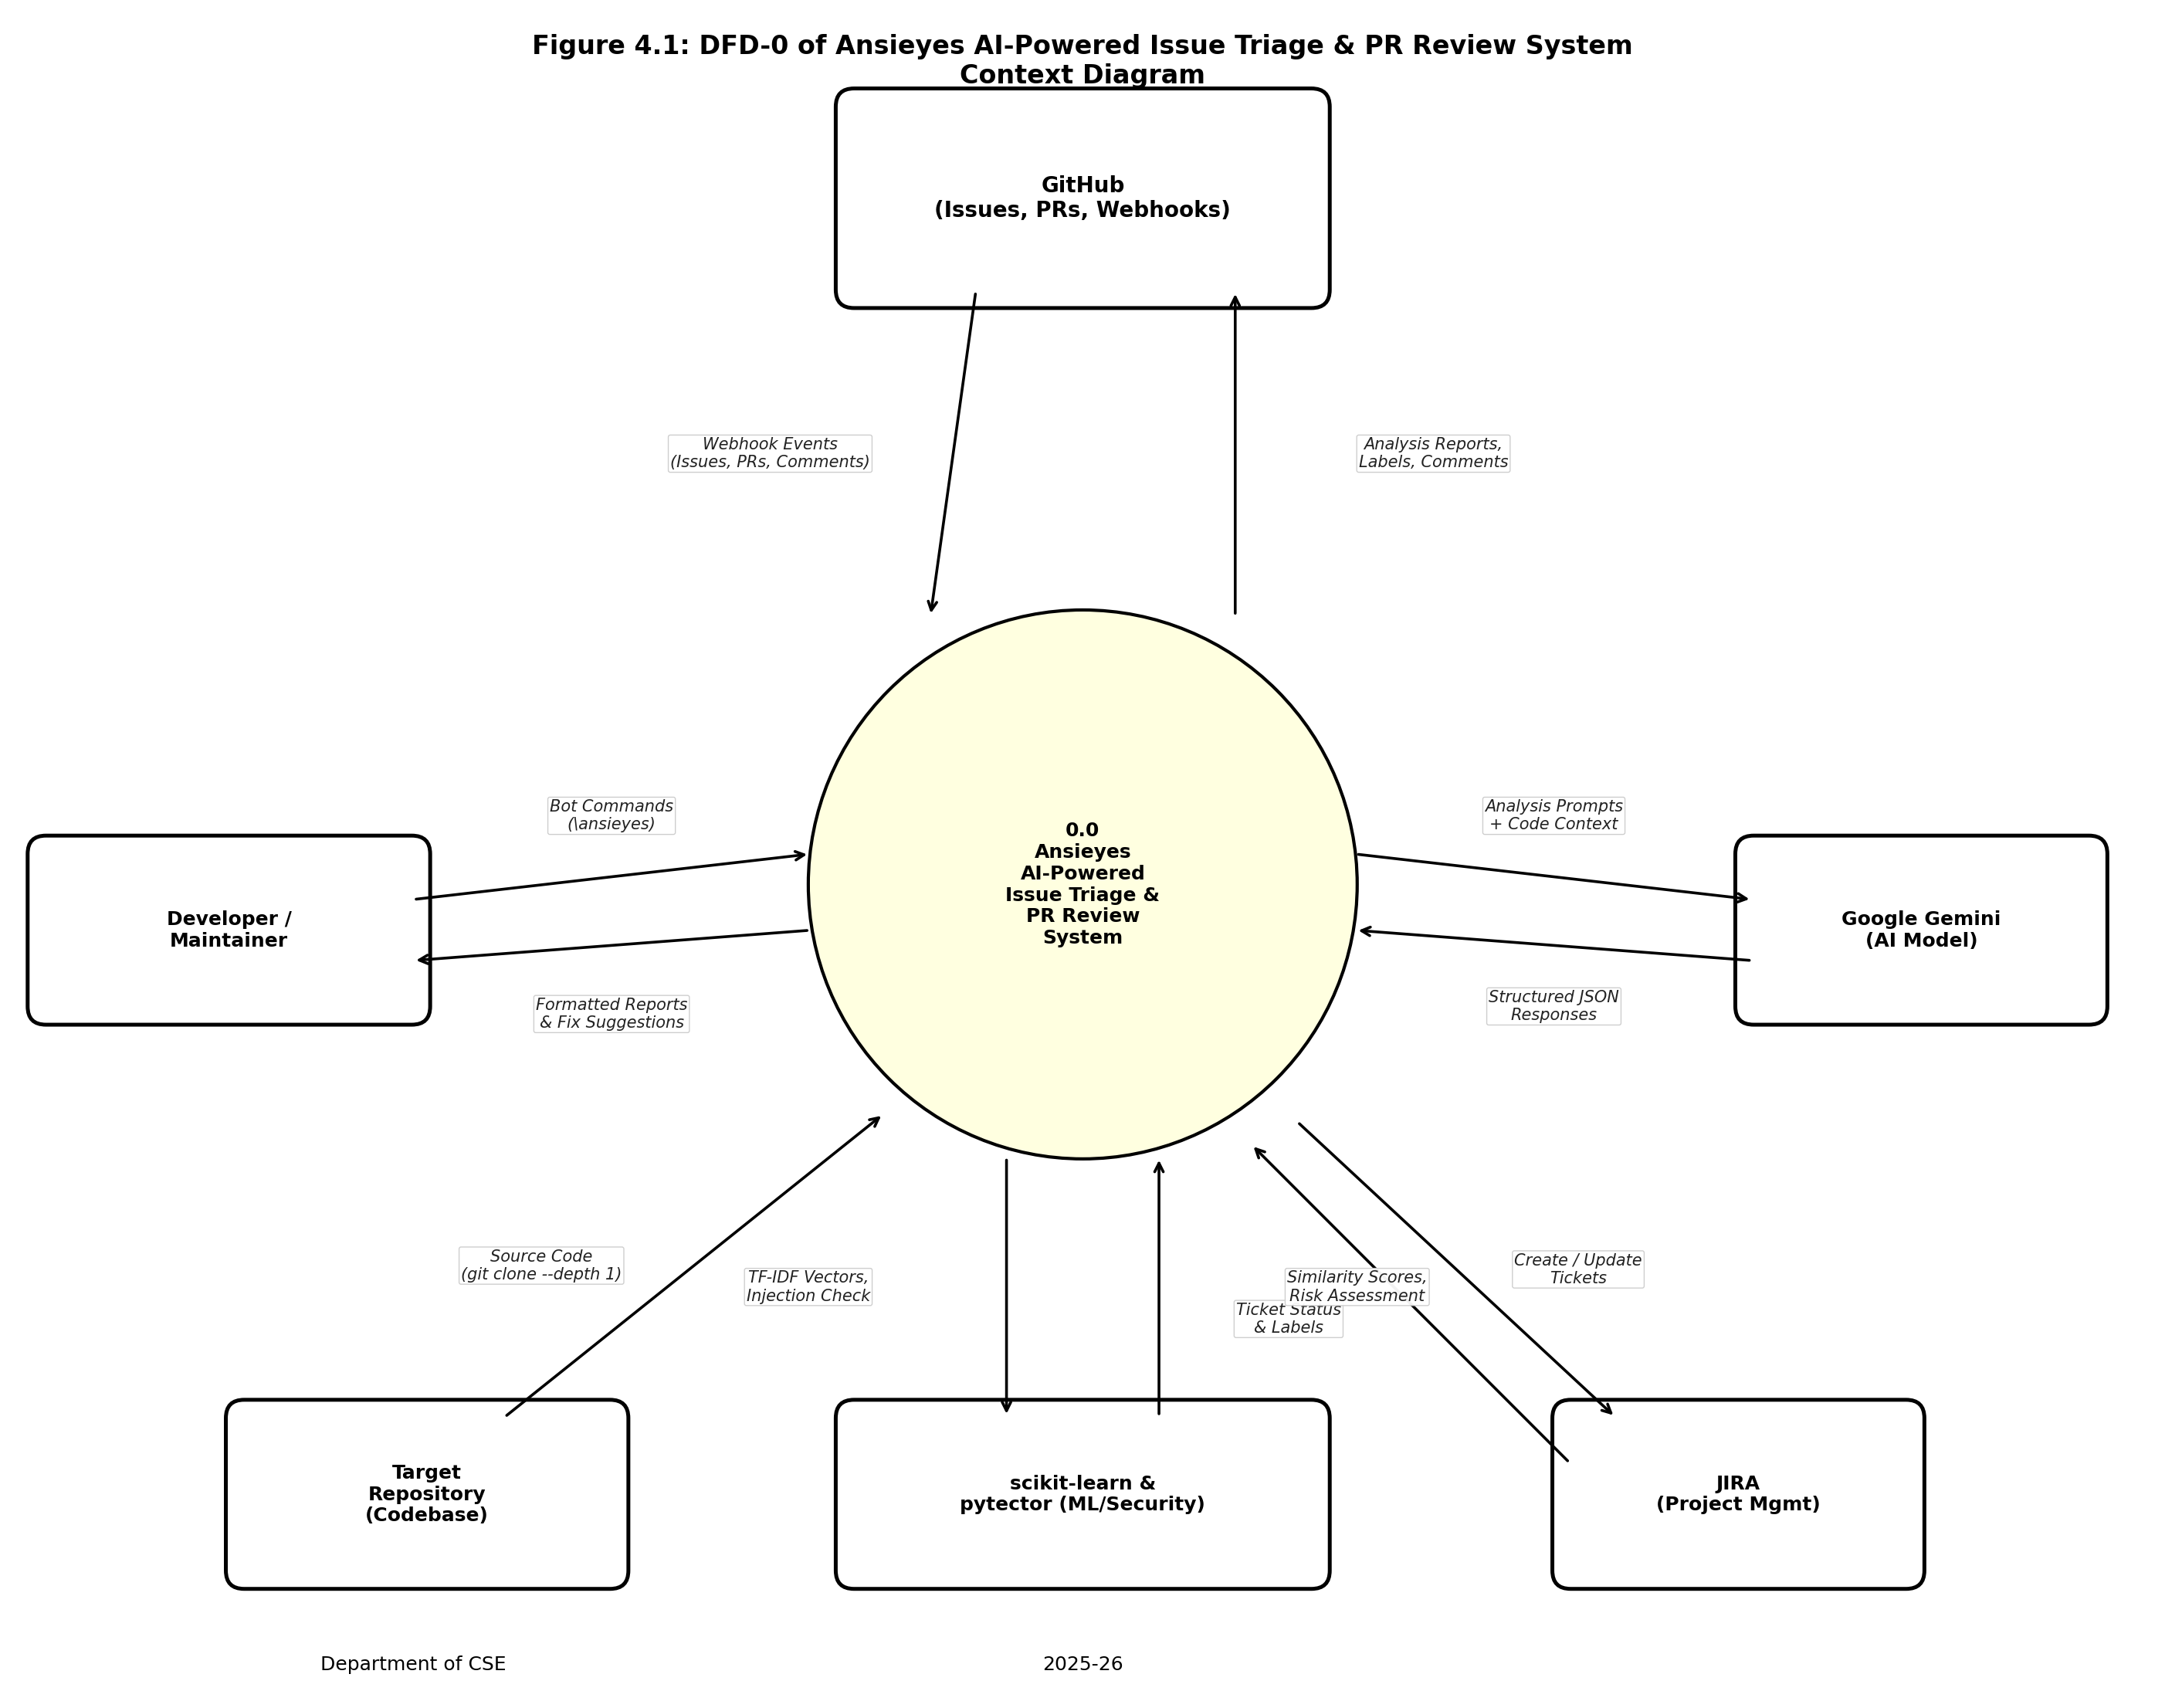
\includegraphics[width=1.0\textwidth]{Figures/report_image_1}
\caption[DFD-0 of Ansieyes AI-Powered Issue Triage and PR Review System Context Diagram]{\textbf{DFD-0 of Ansieyes AI-Powered Issue Triage and PR Review System Context Diagram}}
\vspace{2mm}
\label{fig:dfd0}
\end{figure}

Figure \ref{fig:dfd1} decomposes the system further into its internal processes: the Webhook Handler, Prompt Injection Detector, Duplicate Detector, Issue Triager (Librarian + Surgeon), PR Reviewer, Auto-Fixer, and Output Formatter.

\begin{figure}[htb]
\centering
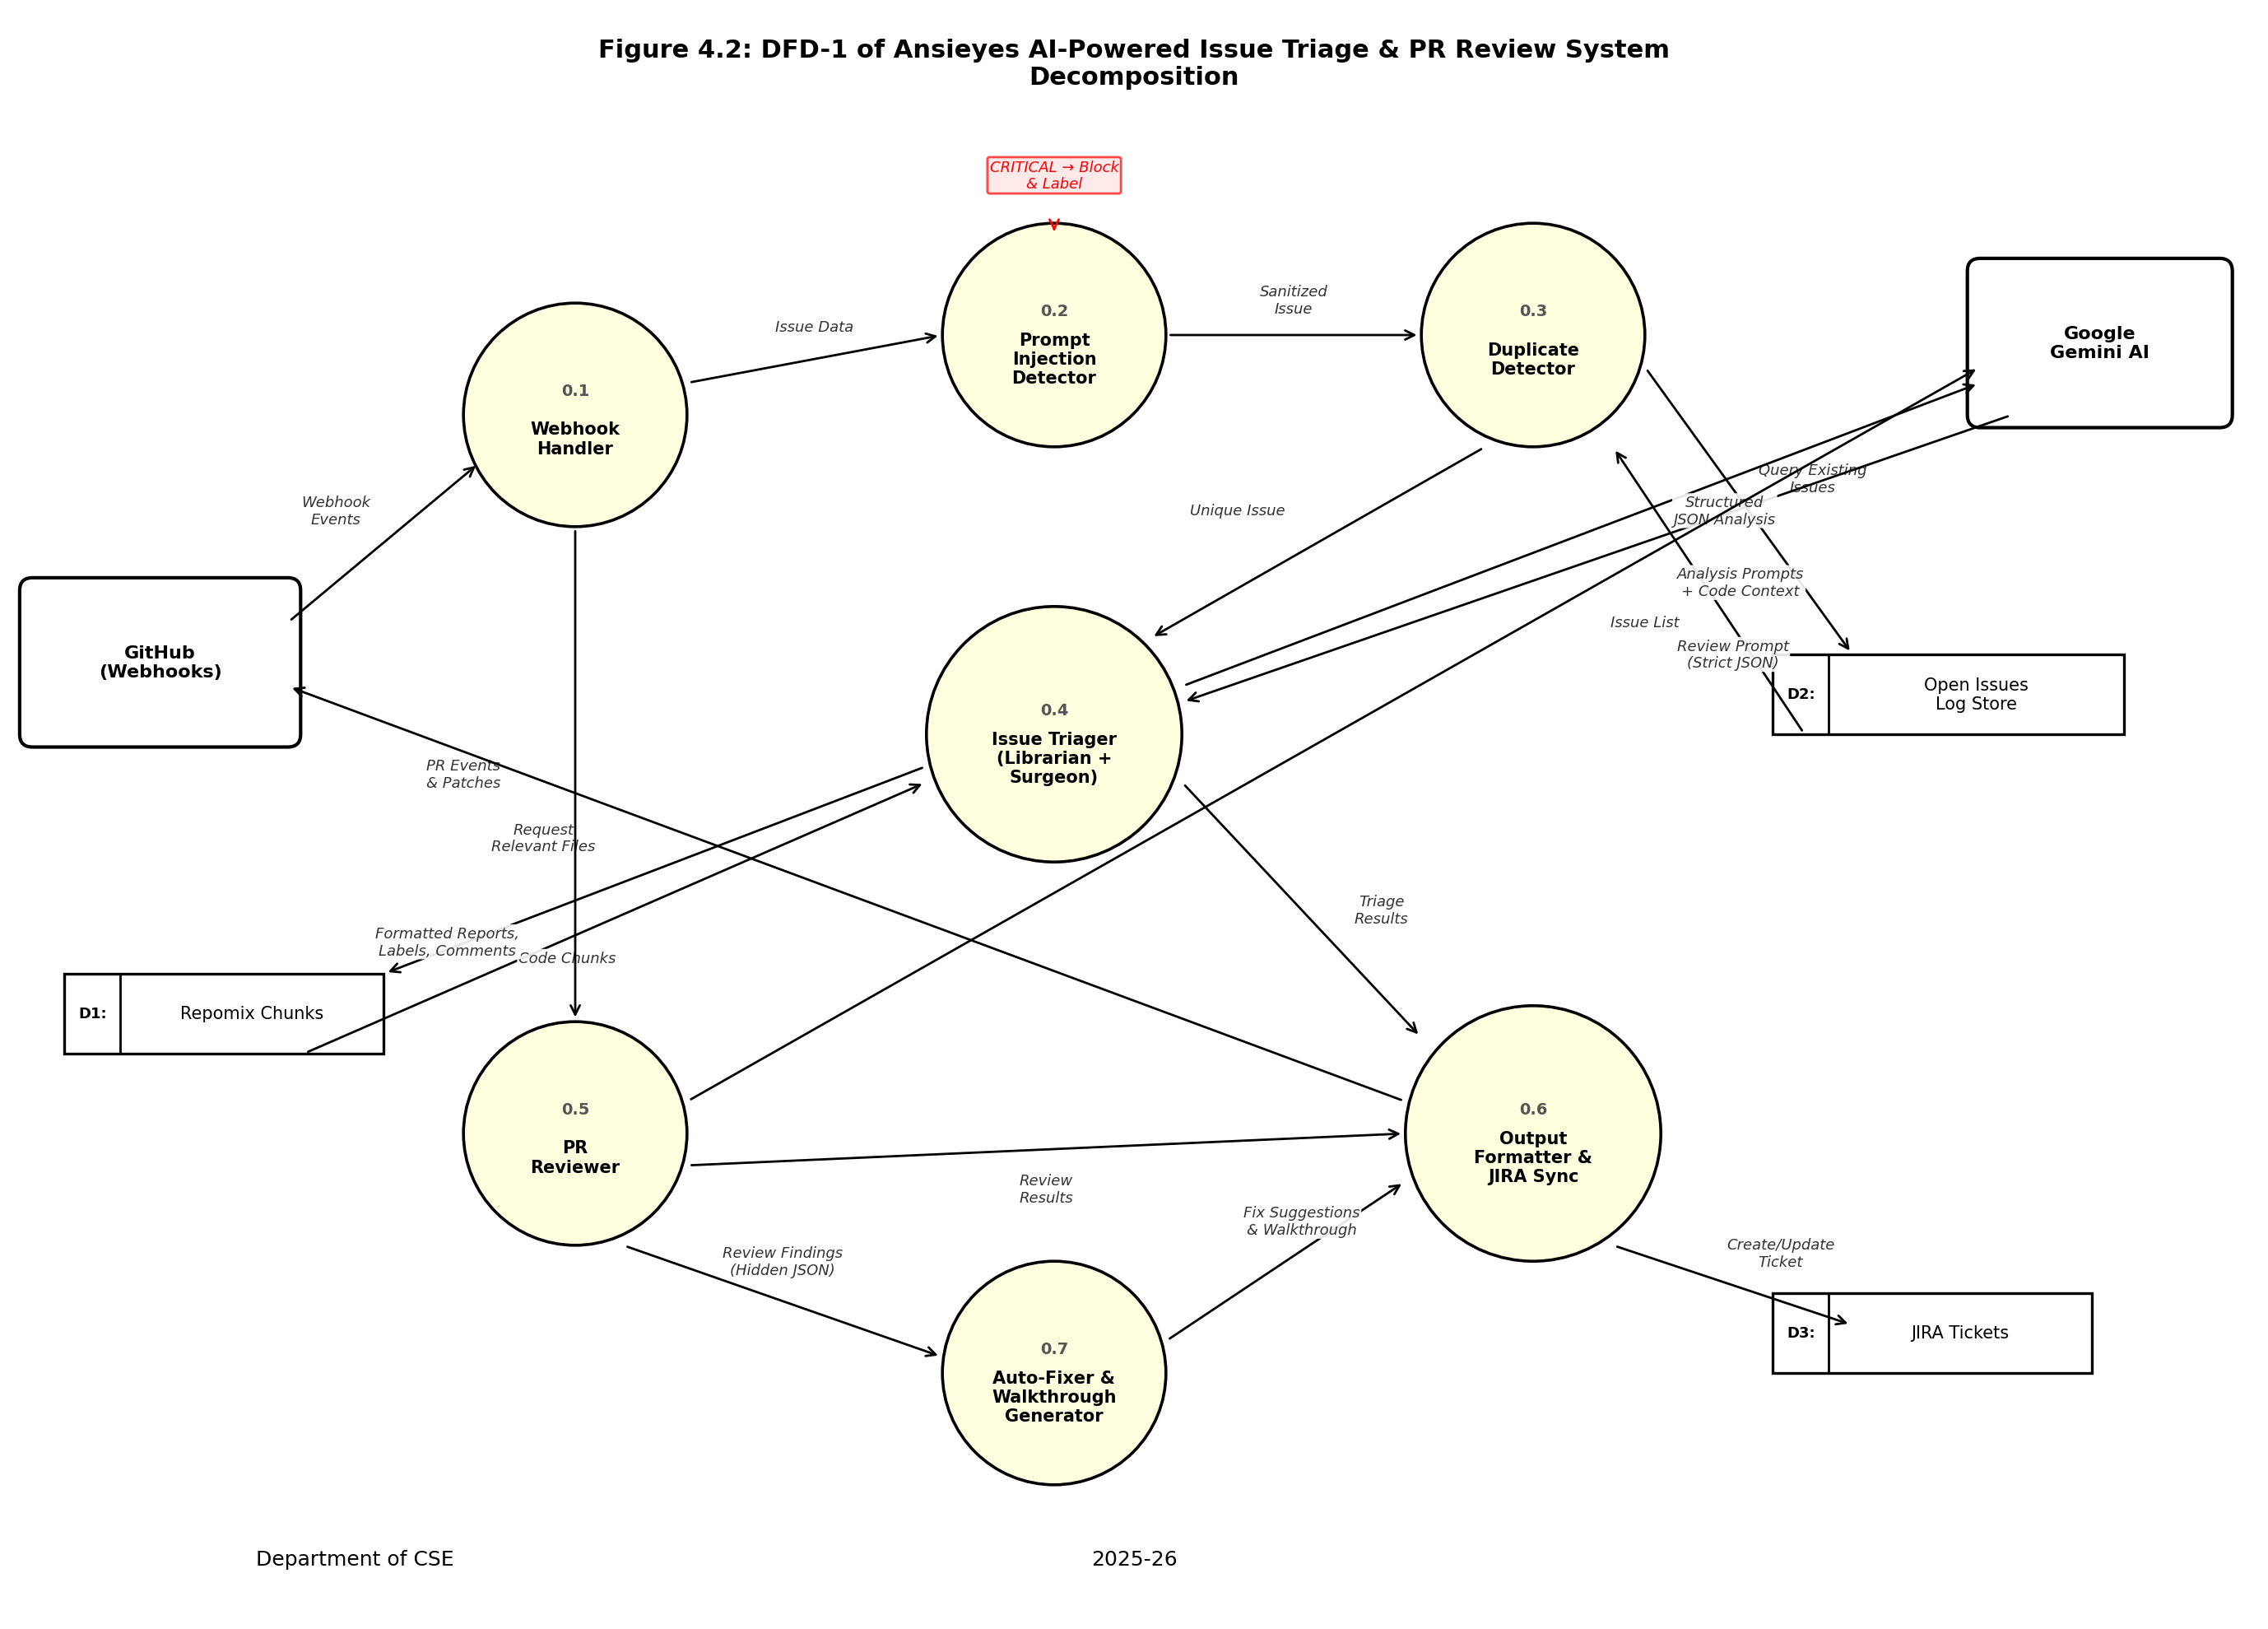
\includegraphics[width=1.0\textwidth]{Figures/report_image_2}
\caption[DFD-1 of Ansieyes AI-Powered Issue Triage and PR Review System Decomposition]{\textbf{DFD-1 of Ansieyes AI-Powered Issue Triage and PR Review System Decomposition}}
\vspace{2mm}
\label{fig:dfd1}
\end{figure}

\subsection{Trigger Layer}
The entry point is a set of GitHub Actions workflows that listen for repository events. When a new issue is created, a workflow fires and kicks off the analysis pipeline. We provide six workflow configurations to suit different team preferences:

\begin{itemize}
\item Analyse every new issue automatically.
\item Analyse only issues with a specific label (to control \gls{api} costs).
\item Bulk re-analyse all open issues after a \gls{pr} merge (so analyses reflect the latest code).
\item Label-filtered bulk analysis.
\item Two-pass analysis using the Librarian--Surgeon pipeline.
\item \gls{pr} review on labelled pull requests.
\end{itemize}

\subsection{Security and Preprocessing Layer}
Every issue passes through this layer before reaching the analyser. It performs three checks: prompt injection detection (described in detail below), input sanitisation to mask any \gls{api} keys or credentials accidentally included in the issue text, and duplicate detection to avoid wasting \gls{api} calls on already-reported problems.

\subsection{Analysis Engine Layer}
Three specialised analysers live in this layer. The GeminiIssueAnalyser (which we call the Surgeon) handles deep issue analysis. The LibrarianAnalyser handles file selection for the two-pass mode. The PRAnalyser provides pull request review with repository-type-specific prompts.

\subsection{Data Models Layer}
All analysis outputs are defined as Pydantic models, which enforce type safety and value constraints at runtime. If the \gls{llm} produces a confidence score outside the 0--1 range, for example, Pydantic catches it before the result reaches the user.

\subsection{Configuration Management}
Rather than hardcoding parameters throughout the codebase, Ansieyes centralises its configuration into two files. The first, \texttt{triage.config.json}, controls the analysis pipeline---it specifies the Gemini model to use, the similarity threshold for duplicate detection, the maximum file count for single-pass mode, and feature flags for enabling or disabling specific modules. The second, \texttt{pr\_prompt\_config.yml}, maps repository URL patterns to specialised \gls{pr} review prompts so that a Python project gets different review criteria than, say, a JavaScript frontend. This separation means that teams can tune Ansieyes for their specific workflow without touching any source code; they simply edit the relevant configuration file and the changes take effect on the next run.

\subsection{Workflow Orchestration}
The six GitHub Actions workflows described in the Trigger Layer do not operate in isolation---they form a coordinated pipeline. The issue analysis workflow triggers first and posts its results as a comment; if duplicate detection is enabled, the duplicate detection workflow runs in parallel and adds a separate label and comment. The bulk re-analysis workflow listens for \gls{pr} merge events and re-triggers analysis on all open issues so that triage results stay current with the latest code. The \gls{pr} review workflow operates on its own event stream. Coordination between these workflows is handled through GitHub's native event system and shared labels, which means no external orchestration service is needed. This design keeps the deployment simple---repository owners just copy the workflow files into their \texttt{.github/workflows} directory and set the required secrets.

\section{Data Model Design}

We defined five core models to represent the system's outputs. Table \ref{tab:models} summarises their key fields.

\begin{table}[htb]
\centering
\renewcommand{\arraystretch}{1.3}
\setlength{\arrayrulewidth}{0.5mm}
\fontsize{10}{12}\selectfont
\caption[Core data models and their fields]{\textbf{Core data models and their fields}}
\vspace{2mm}
\label{tab:models}
\begin{tabular}{|p{3.8cm}|p{8cm}|}
\hline
\textbf{Model} & \textbf{Key Fields} \\
\hline
IssueAnalysis & issue\_type, severity, root\_cause\_analysis, proposed\_solutions, confidence\_score, analysis\_summary \\
\hline
RootCauseAnalysis & primary\_cause, contributing\_factors, affected\_components, related\_code\_locations \\
\hline
CodeSolution & description, code\_changes, location (file, line, function, class), rationale \\
\hline
DuplicateDetectionResult & is\_duplicate, duplicate\_of, similarity\_score, similarity\_reasons, recommendation \\
\hline
InjectionResult & is\_injection, risk\_level, confidence\_score, detected\_patterns, sanitized\_text \\
\hline
\end{tabular}
\end{table}

The IssueAnalysis model deserves a closer look. Its \texttt{issue\_type} field accepts one of three values: bug, enhancement, or feature\_request. The \texttt{severity} field ranges from low to critical. The \texttt{root\_cause\_analysis} is itself a nested object containing the primary cause as text, a list of contributing factors, a list of affected components, and a list of code locations (each with file path, line number, function name, and class name). Proposed solutions follow a similar structure, with each solution specifying where in the code the change should be made and why.

\section{Two-Pass Librarian--Surgeon Architecture}

For small to medium repositories, loading the entire codebase into a single Gemini prompt works well. But enterprise-scale projects can have hundreds of thousands of lines of code, far more than the model can process at once. Even for projects that technically fit, stuffing irrelevant code into the context dilutes the model's attention and wastes tokens.

Our solution splits the analysis into two passes, as shown in Figure \ref{fig:twopass}.

\begin{figure}[htb]
\centering
\begin{tikzpicture}[
    node distance=0.8cm,
    block/.style={rectangle, draw, fill=blue!8, text width=5cm, minimum height=1cm, align=center, rounded corners=2pt, font=\small},
    data/.style={rectangle, draw, fill=orange!10, text width=5cm, minimum height=0.8cm, align=center, rounded corners=2pt, font=\small\itshape},
    arrow/.style={-{Stealth[length=2.5mm]}, thick}
]
\node[data] (input) {Issue Title + Description};
\node[block, below=of input] (lib) {\textbf{Pass 1: Librarian}\\Analyse directory chunks};
\node[data, below=of lib] (files) {List of Relevant Files};
\node[block, below=of files] (repomix) {Generate Targeted Repomix};
\node[data, below=of repomix] (context) {Focused Codebase Context};
\node[block, below=of context] (surgeon) {\textbf{Pass 2: Surgeon}\\Deep issue analysis};
\node[data, below=of surgeon] (output) {Structured Analysis Output};

\draw[arrow] (input) -- (lib);
\draw[arrow] (lib) -- (files);
\draw[arrow] (files) -- (repomix);
\draw[arrow] (repomix) -- (context);
\draw[arrow] (context) -- (surgeon);
\draw[arrow] (surgeon) -- (output);
\end{tikzpicture}
\caption[Two-pass Librarian--Surgeon flow]{\textbf{Two-pass Librarian--Surgeon flow}}
\vspace{2mm}
\label{fig:twopass}
\end{figure}

\subsection{Pass 1: The Librarian}
The Librarian receives the issue description along with a set of directory-level ``chunks''---compressed summaries of each top-level directory in the repository. For each chunk, it asks Gemini: \textit{which files in this directory are relevant to the reported issue?} The model returns a list of file paths, which the Librarian validates (discarding paths that lack a file extension, exceed 200 characters, or start with comment markers). A dependency analysis step can optionally include files imported by the initially identified set.

\subsection{Pass 2: The Surgeon}
A new Repomix output is generated containing only the files the Librarian identified. The Surgeon---which is just the standard GeminiIssueAnalyser---runs its full analysis against this focused context. Because it is working with a fraction of the original codebase, the analysis is both cheaper and more precise.

\subsection{Token Savings}
If a repository has $N$ files in total and the Librarian selects $R$ of them, the token reduction is approximately $1 - R/N$. In practice, we observed reductions between 57\% and 70\% on medium to large repositories. For very large codebases that exceed the single-pass context limit entirely, the two-pass approach is the only option.

\section{Security Architecture}

We designed the security module as three independent detectors whose outputs are aggregated. Figure \ref{fig:security} illustrates the pipeline.

\begin{figure}[htb]
\centering
\begin{tikzpicture}[
    node distance=0.6cm and 1.5cm,
    block/.style={rectangle, draw, fill=blue!8, text width=3.2cm, minimum height=1cm, align=center, rounded corners=2pt, font=\small},
    input/.style={rectangle, draw, fill=orange!10, text width=3.5cm, minimum height=0.8cm, align=center, rounded corners=2pt, font=\small\itshape},
    output/.style={rectangle, draw, fill=green!10, text width=3.5cm, minimum height=0.8cm, align=center, rounded corners=2pt, font=\small},
    arrow/.style={-{Stealth[length=2.5mm]}, thick}
]
\node[input] (input) {Issue Description};
\node[block, below left=1cm and 0.3cm of input] (ml) {ML-Based\\Detector};
\node[block, below=1cm of input] (pattern) {Pattern\\Matching};
\node[block, below right=1cm and 0.3cm of input] (heuristic) {Heuristic\\Analysis};
\node[block, below=2.8cm of input] (agg) {Risk Aggregation};
\node[output, below=of agg] (result) {Risk Level + Confidence};

\draw[arrow] (input) -- (ml);
\draw[arrow] (input) -- (pattern);
\draw[arrow] (input) -- (heuristic);
\draw[arrow] (ml) -- (agg);
\draw[arrow] (pattern) -- (agg);
\draw[arrow] (heuristic) -- (agg);
\draw[arrow] (agg) -- (result);
\end{tikzpicture}
\caption[Multi-layered prompt injection detection pipeline]{\textbf{Multi-layered prompt injection detection pipeline}}
\vspace{2mm}
\label{fig:security}
\end{figure}

The aggregator takes the highest risk level reported by any individual detector. This conservative strategy means that even if an attacker manages to slip past one layer, the others can still catch the attempt. Risk levels range from Safe through Low, Medium, and High to Critical. Issues flagged as High or Critical are blocked from analysis entirely; Low and Medium risks proceed with a warning.

\section{Duplicate Detection Design}

We offer two approaches, each with its own trade-offs.

The \textbf{Gemini-based} detector sends the new issue along with all existing open issues to the model and asks it to evaluate semantic similarity. It can catch duplicates even when the wording is completely different---for example, one issue saying ``the app crashes on login'' and another saying ``authentication module throws a null pointer exception.'' The downside is that each check costs an \gls{api} call.

The \textbf{cosine similarity} detector works offline. It preprocesses issue text (lowercasing, removing special characters), builds \gls{tfidf} vectors with unigram and bigram features, and computes cosine similarity. We weight the title 2x relative to the description, since titles tend to carry the most distinctive information. Issues above a 0.6 similarity threshold are flagged. This method is fast (under 100 milliseconds) but misses semantic duplicates that use different words.

\section{PR Review Design}

The pull request reviewer extends Ansieyes to code review. It uses a \gls{yaml} configuration file that maps repository URL patterns (for example, repositories with ``python'' in the name) to specialised review prompts. The reviewer analyses the \gls{pr} diff, generates file-specific comments with line numbers, and produces an overall assessment broken into strengths, issues, and suggestions.

The design choices described in this chapter were shaped by practical constraints: \gls{api} costs, context window limits, and the need to handle adversarial inputs. The next chapter explains how we turned these designs into working code.

\section{Summary}

This chapter described the high-level design of Ansieyes, covering its four-layer architecture, data model design, the two-pass Librarian--Surgeon strategy for scaling to large codebases, the multi-layered security pipeline for prompt injection defence, the dual duplicate detection approach, and the PR review subsystem. These design decisions translate the theoretical foundations from the previous chapter into a concrete system structure that the next chapter implements.


		%Chapter 5
		\chapter{Detailed Design of Ansieyes}

The high-level design presented in the previous chapter described the overall architecture and the relationships between the major components. This chapter goes deeper into the module-level design, explaining the internal structure of each component, the data flow between them, and the design decisions that shaped their implementation.

\section{Architectural Design}

Ansieyes is organised around five core modules that work together to process a GitHub issue from the moment it is received to the point where a structured analysis is posted back as a comment. Figure \ref{fig:structure_chart} shows the module hierarchy.

\begin{figure}[htb]
\centering
\begin{tikzpicture}[
    node distance=1.2cm and 0.8cm,
    module/.style={rectangle, draw, fill=blue!8, text width=3cm, minimum height=1cm, align=center, rounded corners=2pt, font=\small},
    arrow/.style={-{Stealth[length=2.5mm]}, thick}
]
\node[module] (main) {Ansieyes Core};
\node[module, below left=1.5cm and 2cm of main] (security) {Security\\Module};
\node[module, below left=1.5cm and -0.5cm of main] (duplicate) {Duplicate\\Detection};
\node[module, below right=1.5cm and -0.5cm of main] (analyzer) {Issue\\Analyzer};
\node[module, below right=1.5cm and 2cm of main] (pr) {PR\\Reviewer};
\node[module, below=3cm of main] (librarian) {Librarian-\\Surgeon};

\draw[arrow] (main) -- (security);
\draw[arrow] (main) -- (duplicate);
\draw[arrow] (main) -- (analyzer);
\draw[arrow] (main) -- (pr);
\draw[arrow] (main) -- (librarian);
\draw[arrow] (librarian) -- (analyzer);
\end{tikzpicture}
\caption[Structure chart of Ansieyes modules]{\textbf{Structure chart of Ansieyes modules}}
\label{fig:structure_chart}
\end{figure}

Each incoming issue passes through the Security Module first, then the Duplicate Detection Module, and finally reaches either the Issue Analyzer (for single-pass analysis) or the Librarian-Surgeon pipeline (for large repositories). The PR Reviewer operates independently on pull request events.

\section{Structure Chart}

The structure chart in Figure \ref{fig:structure_chart} illustrates the hierarchical decomposition of the system. The Ansieyes Core acts as the orchestrator, dispatching work to the appropriate module based on the event type and the results of upstream checks. The Security Module and Duplicate Detection Module act as filters: if either flags the input as unsafe or redundant, the pipeline terminates early without invoking the computationally expensive analyzer.

\section{Module Overview}

The system comprises five functional modules:

\begin{enumerate}
\item \textbf{Security Module} -- Screens all incoming issue text for prompt injection attacks using three detection layers.
\item \textbf{Duplicate Detection Module} -- Checks whether the issue has already been reported, using both semantic and statistical methods.
\item \textbf{Issue Analysis Module} -- Performs deep analysis of the issue against the repository's source code.
\item \textbf{Librarian-Surgeon Module} -- Handles large repositories by first selecting relevant files, then running targeted analysis.
\item \textbf{PR Review Module} -- Provides automated code review for pull requests.
\end{enumerate}

\section{Issue Analysis Module}

The Issue Analysis Module is built around the \texttt{GeminiIssueAnalyzer} class. When invoked, it loads the repository's source code from a Repomix output file, constructs a detailed prompt combining the issue title, description, and codebase content, and sends this to the Gemini \gls{api}. The response is parsed through a three-strategy extraction pipeline: first attempting to extract \gls{json} from markdown code blocks, then using a brace-counting parser, and finally falling back to greedy regex matching. If structured extraction fails entirely, a pattern-based text extractor recovers the key fields from the raw response.

Every parsed result undergoes quality validation before being accepted. The validator checks for a minimum number of proposed solutions, a confidence score above 0.3, the absence of placeholder file paths, and minimum lengths for the analysis summary and primary cause fields. If the result fails validation, the module retries with the same prompt up to a configurable number of times (default: two retries).

\section{Security Module}

The Security Module implements a three-layer detection pipeline. The first layer uses the pytector library, a pre-trained \gls{ml} model that classifies text as safe or potentially injected. The second layer applies compiled regular expressions across seven categories: role manipulation, system prompt injection, instruction bypass, file manipulation, code injection, data extraction, and prompt leakage. Each category carries a predefined confidence weight, with instruction bypass receiving the highest weight (0.95) and file manipulation the lowest (0.75). The third layer performs heuristic analysis, checking for statistical anomalies such as excessive special character sequences, unusually high counts of instruction-like keywords, suspicious formatting patterns, and abnormally long sentences.

The aggregation logic takes the maximum confidence score across all three layers and counts the total number of unique patterns detected. Risk levels are assigned based on these two values: Critical for confidence above 0.9 or five or more patterns, High for confidence above 0.8 or three or more patterns, and so on down to Safe. Issues flagged as High or Critical are blocked from analysis; the offending text is sanitised and a security alert is posted on the issue.

\section{Duplicate Detection Module}

The duplicate detection subsystem offers two complementary approaches. The Gemini-based detector sends the new issue alongside all existing open issues to the \gls{llm} and asks it to evaluate semantic similarity across five dimensions: symptoms, root cause, affected components, user impact, and technical context. The prompt explicitly instructs the model to prefer not marking an issue as duplicate when uncertain, which reduces false positives at the cost of slightly lower recall.

The cosine similarity detector operates entirely offline. It preprocesses issue text by converting to lowercase, removing special characters, and normalising whitespace. Each issue is represented as a \gls{tfidf} vector using unigrams and bigrams with a maximum of 5,000 features. The title is weighted twice relative to the description, since titles tend to carry the most distinctive information. Cosine similarity is computed between the new issue vector and all existing issue vectors, and any match above the configurable threshold (default: 0.6) is flagged as a potential duplicate.

\section{Librarian-Surgeon Module}

For repositories that exceed the \gls{llm}'s context window, the Librarian-Surgeon module splits the analysis into two passes. The Librarian loads directory-level chunks from the repository and asks Gemini to identify which directories and files are relevant to the reported issue. Returned file paths are validated against several criteria: they must contain a directory separator, have a file extension, not start with a comment marker, and not exceed 200 characters.

Once the Librarian produces a validated file list, a targeted Repomix output is generated containing only those files. The Surgeon -- which is the standard GeminiIssueAnalyzer -- then runs its full analysis pipeline against this focused context. The net effect is a significant reduction in token consumption (57--70\% for medium to large repositories) with improved analysis precision, since the model's attention is not diluted by irrelevant code.

\section{PR Review Module}

The PR Review Module is built around the \texttt{PRAnalyzer} class. It uses a \gls{yaml} configuration file that maps repository URL patterns to domain-specific review prompts. For example, repositories matching a Python-related pattern receive prompts emphasising PEP 8 compliance and docstring coverage, while \gls{ai}/\gls{ml} repositories get prompts focused on model validation and data handling.

The reviewer processes the \gls{pr} diff, generates file-specific comments with line numbers, and produces an overall assessment broken into strengths, issues found, and suggestions. It also supports workflow analysis, where it can diagnose GitHub Actions failures by examining job logs and step outputs.

\section{Summary}

This chapter presented the detailed module-level design of Ansieyes. Each of the five modules -- Security, Duplicate Detection, Issue Analysis, Librarian-Surgeon, and PR Review -- was described in terms of its internal logic, data flow, and design rationale. The modular structure ensures that individual components can be tested, maintained, and extended independently. The next chapter describes how these designs were implemented in code.


		%Chapter 6
		\chapter{Implementation of Ansieyes}

With the architecture defined, we moved to implementation. The entire system is written in Python and packaged for installation via pip. In this chapter, we describe the key algorithms and integration details. Due to confidentiality considerations, we present the logic in algorithmic form rather than as raw source code.

\section{Project Organisation}

Table \ref{tab:projstructure} lists the main directories and their roles.

\begin{table}[htb]
\centering
\renewcommand{\arraystretch}{1.3}
\setlength{\arrayrulewidth}{0.5mm}
\fontsize{10}{12}\selectfont
\caption[Project directory layout]{\textbf{Project directory layout}}
\vspace{2mm}
\label{tab:projstructure}
\begin{tabular}{|p{3.5cm}|p{8cm}|}
\hline
\textbf{Directory} & \textbf{Role} \\
\hline
\texttt{utils/} & Core library: analyser, models, security, duplicates \\
\hline
\texttt{cli/} & Command-line tools for all features \\
\hline
\texttt{tests/} & Unit and integration test suite \\
\hline
\texttt{cutlery/workflows/} & GitHub Actions workflow templates \\
\hline
\texttt{ui/} & Streamlit-based web interface (prototype) \\
\hline
\end{tabular}
\end{table}

After installation, four commands become available: \texttt{ai-triage} for issue analysis, \texttt{ai-triage-duplicate} for duplicate detection, \texttt{ai-triage-cosine} for offline similarity checking, and \texttt{ai-triage-pr} for pull request review.

\section{Core Analysis Engine}

The central class, \texttt{GeminiIssueAnalyser}, orchestrates the full analysis pipeline. Algorithm \ref{alg:analyse} outlines the process.

\begin{figure}[htb]
\centering
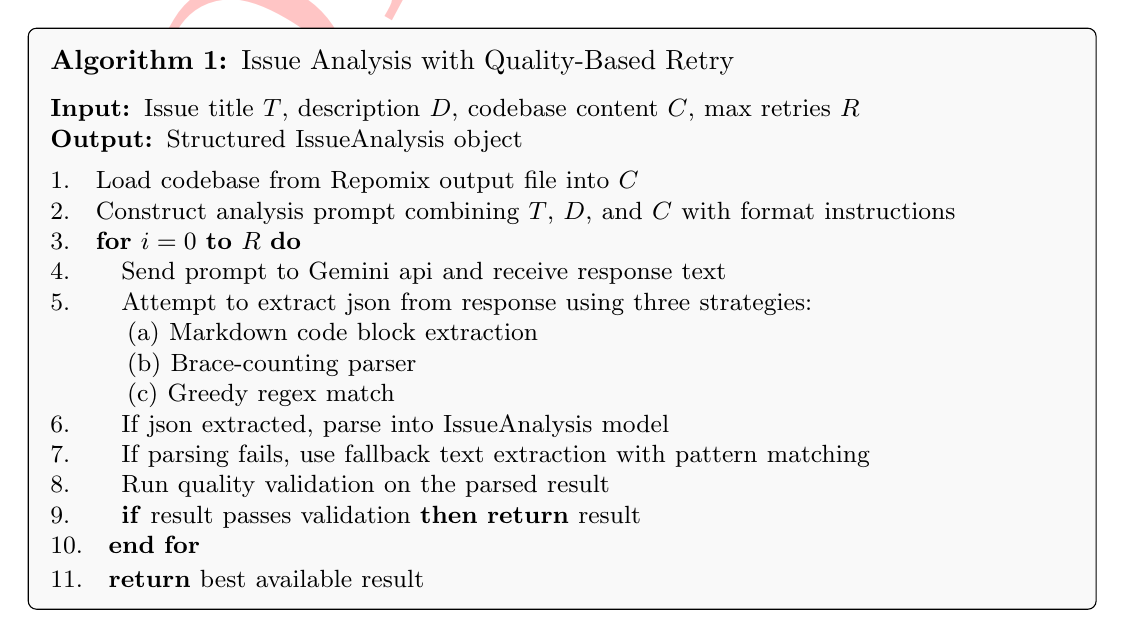
\begin{tikzpicture}
\node[draw, text width=13cm, inner sep=8pt, rounded corners=3pt, fill=gray!5] {
\textbf{Algorithm 1:} Issue Analysis with Quality-Based Retry\\[6pt]
\small
\textbf{Input:} Issue title $T$, description $D$, codebase content $C$, max retries $R$\\
\textbf{Output:} Structured IssueAnalysis object\\[4pt]
1.\quad Load codebase from Repomix output file into $C$\\
2.\quad Construct analysis prompt combining $T$, $D$, and $C$ with format instructions\\
3.\quad \textbf{for} $i = 0$ \textbf{to} $R$ \textbf{do}\\
4.\quad\quad Send prompt to Gemini \gls{api} and receive response text\\
5.\quad\quad Attempt to extract \gls{json} from response using three strategies:\\
\quad\quad\quad (a) Markdown code block extraction\\
\quad\quad\quad (b) Brace-counting parser\\
\quad\quad\quad (c) Greedy regex match\\
6.\quad\quad If \gls{json} extracted, parse into IssueAnalysis model\\
7.\quad\quad If parsing fails, use fallback text extraction with pattern matching\\
8.\quad\quad Run quality validation on the parsed result\\
9.\quad\quad \textbf{if} result passes validation \textbf{then return} result\\
10.\quad \textbf{end for}\\
11.\quad \textbf{return} best available result
};
\end{tikzpicture}
\label{alg:analyse}
\end{figure}

\subsection{Quality Validation}
We found early on that the model occasionally produces vague or incomplete analyses, especially for issues with sparse descriptions. To catch these, we run every response through a validation check before accepting it. An analysis is considered low quality if any of the following are true:

\begin{itemize}
\item It contains fewer than one proposed solution.
\item The confidence score is below 0.3.
\item File paths include placeholder text such as ``path/to/'' or ``example.py.''
\item The analysis summary is shorter than 20 characters.
\item The primary cause description is shorter than 10 characters.
\item Any solution description is shorter than 10 characters.
\end{itemize}

If a response fails this check, the system retries with the same prompt, up to a configurable limit (default: 2 retries). In our testing, most low-quality responses were corrected on the first retry.

\subsection{Prompt Design}
The analysis prompt is built from four parts: a system role statement (``You are an expert software engineer analysing a code issue''), the issue title and description, the full codebase content, and detailed instructions specifying the expected \gls{json} output format. We also include guidelines telling the model to use diff-style code changes, reference actual files from the codebase, and acknowledge when it is uncertain rather than guessing.

Custom prompts can be loaded from a file, allowing teams to tailor the analysis for their specific domain or conventions.

\section{Prompt Injection Detection}

The security module runs before any issue reaches the analyser. Algorithm \ref{alg:injection} describes the multi-layered detection process.

\begin{figure}[htb]
\centering
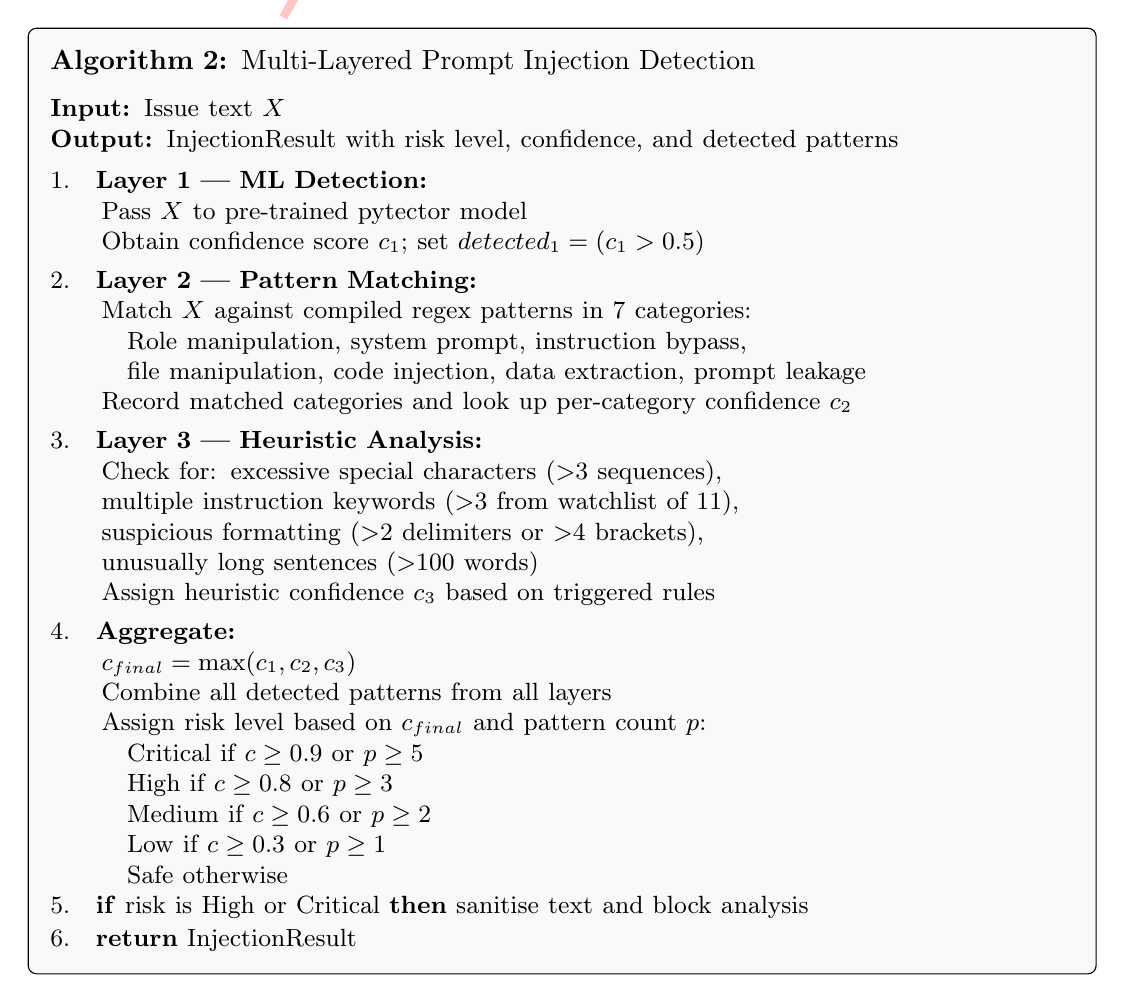
\begin{tikzpicture}
\node[draw, text width=13cm, inner sep=8pt, rounded corners=3pt, fill=gray!5] {
\textbf{Algorithm 2:} Multi-Layered Prompt Injection Detection\\[6pt]
\small
\textbf{Input:} Issue text $X$\\
\textbf{Output:} InjectionResult with risk level, confidence, and detected patterns\\[4pt]
1.\quad \textbf{Layer 1 --- ML Detection:}\\
\quad\quad Pass $X$ to pre-trained pytector model\\
\quad\quad Obtain confidence score $c_1$; set $\text{detected}_1 = (c_1 > 0.5)$\\[3pt]
2.\quad \textbf{Layer 2 --- Pattern Matching:}\\
\quad\quad Match $X$ against compiled regex patterns in 7 categories:\\
\quad\quad\quad Role manipulation, system prompt, instruction bypass,\\
\quad\quad\quad file manipulation, code injection, data extraction, prompt leakage\\
\quad\quad Record matched categories and look up per-category confidence $c_2$\\[3pt]
3.\quad \textbf{Layer 3 --- Heuristic Analysis:}\\
\quad\quad Check for: excessive special characters ($>$3 sequences),\\
\quad\quad multiple instruction keywords ($>$3 from watchlist of 11),\\
\quad\quad suspicious formatting ($>$2 delimiters or $>$4 brackets),\\
\quad\quad unusually long sentences ($>$100 words)\\
\quad\quad Assign heuristic confidence $c_3$ based on triggered rules\\[3pt]
4.\quad \textbf{Aggregate:}\\
\quad\quad $c_{\text{final}} = \max(c_1, c_2, c_3)$\\
\quad\quad Combine all detected patterns from all layers\\
\quad\quad Assign risk level based on $c_{\text{final}}$ and pattern count $p$:\\
\quad\quad\quad Critical if $c \geq 0.9$ or $p \geq 5$\\
\quad\quad\quad High if $c \geq 0.8$ or $p \geq 3$\\
\quad\quad\quad Medium if $c \geq 0.6$ or $p \geq 2$\\
\quad\quad\quad Low if $c \geq 0.3$ or $p \geq 1$\\
\quad\quad\quad Safe otherwise\\
5.\quad \textbf{if} risk is High or Critical \textbf{then} sanitise text and block analysis\\
6.\quad \textbf{return} InjectionResult
};
\end{tikzpicture}
\label{alg:injection}
\end{figure}

The pattern matching layer deserves some additional detail. Table \ref{tab:patterns} lists the seven categories and representative patterns.

\begin{table}[htb]
\centering
\renewcommand{\arraystretch}{1.3}
\setlength{\arrayrulewidth}{0.5mm}
\fontsize{10}{12}\selectfont
\caption[Prompt injection pattern categories and assigned confidence levels]{\textbf{Prompt injection pattern categories and assigned confidence levels}}
\vspace{2mm}
\label{tab:patterns}
\begin{tabular}{|p{3cm}|p{5.5cm}|c|}
\hline
\textbf{Category} & \textbf{Example Patterns} & \textbf{Confidence} \\
\hline
Instruction bypass & ``bypass security,'' ``jailbreak'' & 0.95 \\
\hline
Role manipulation & ``ignore previous instructions,'' ``you are now'' & 0.90 \\
\hline
Prompt leakage & ``show original prompt,'' ``reveal system prompt'' & 0.90 \\
\hline
Code injection & ``eval(,'' ``exec(,'' \texttt{<script>} & 0.85 \\
\hline
System prompts & ``system:,'' ``[system],'' \texttt{```system} & 0.80 \\
\hline
Data extraction & ``show password,'' ``reveal token'' & 0.80 \\
\hline
File manipulation & ``create file,'' ``write to file'' & 0.75 \\
\hline
\end{tabular}
\end{table}

The heuristic layer watches for 11 specific keywords: \textit{ignore, forget, disregard, override, bypass, system, assistant, admin, root, jailbreak, unrestricted}. Seeing three or more of these in a single issue raises the heuristic confidence to 0.7.

\section{Duplicate Detection}

\subsection{Gemini-Based Detection}
Algorithm \ref{alg:geminidup} describes the semantic approach.

\begin{figure}[htb]
\centering
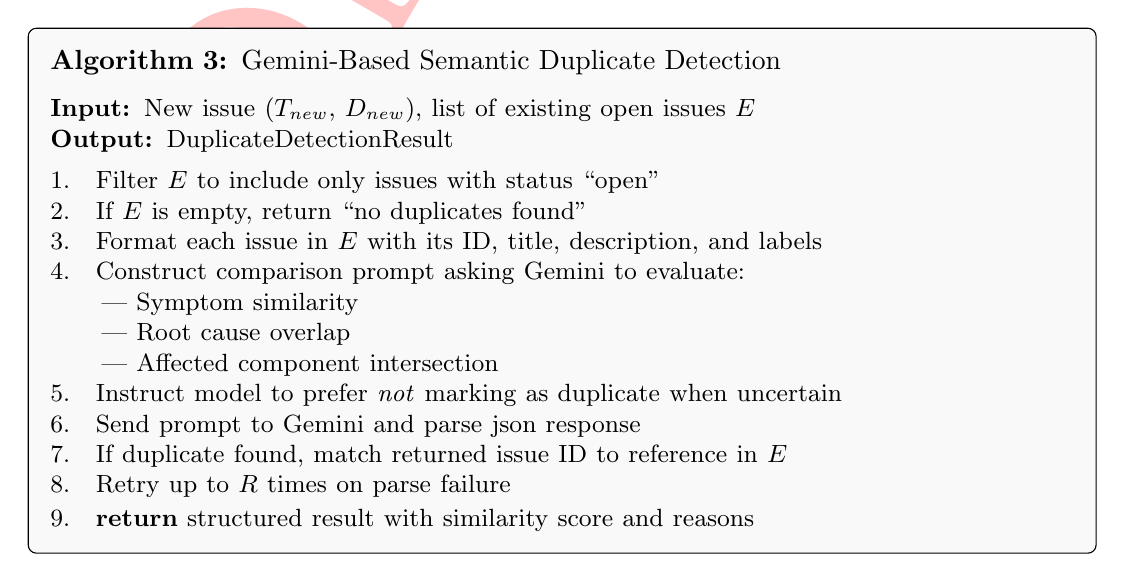
\begin{tikzpicture}
\node[draw, text width=13cm, inner sep=8pt, rounded corners=3pt, fill=gray!5] {
\textbf{Algorithm 3:} Gemini-Based Semantic Duplicate Detection\\[6pt]
\small
\textbf{Input:} New issue ($T_{\text{new}}$, $D_{\text{new}}$), list of existing open issues $E$\\
\textbf{Output:} DuplicateDetectionResult\\[4pt]
1.\quad Filter $E$ to include only issues with status ``open''\\
2.\quad If $E$ is empty, return ``no duplicates found''\\
3.\quad Format each issue in $E$ with its ID, title, description, and labels\\
4.\quad Construct comparison prompt asking Gemini to evaluate:\\
\quad\quad --- Symptom similarity\\
\quad\quad --- Root cause overlap\\
\quad\quad --- Affected component intersection\\
5.\quad Instruct model to prefer \textit{not} marking as duplicate when uncertain\\
6.\quad Send prompt to Gemini and parse \gls{json} response\\
7.\quad If duplicate found, match returned issue ID to reference in $E$\\
8.\quad Retry up to $R$ times on parse failure\\
9.\quad \textbf{return} structured result with similarity score and reasons
};
\end{tikzpicture}
\label{alg:geminidup}
\end{figure}

\subsection{Cosine Similarity Detection}
Algorithm \ref{alg:cosinedup} describes the offline approach.

\begin{figure}[htb]
\centering
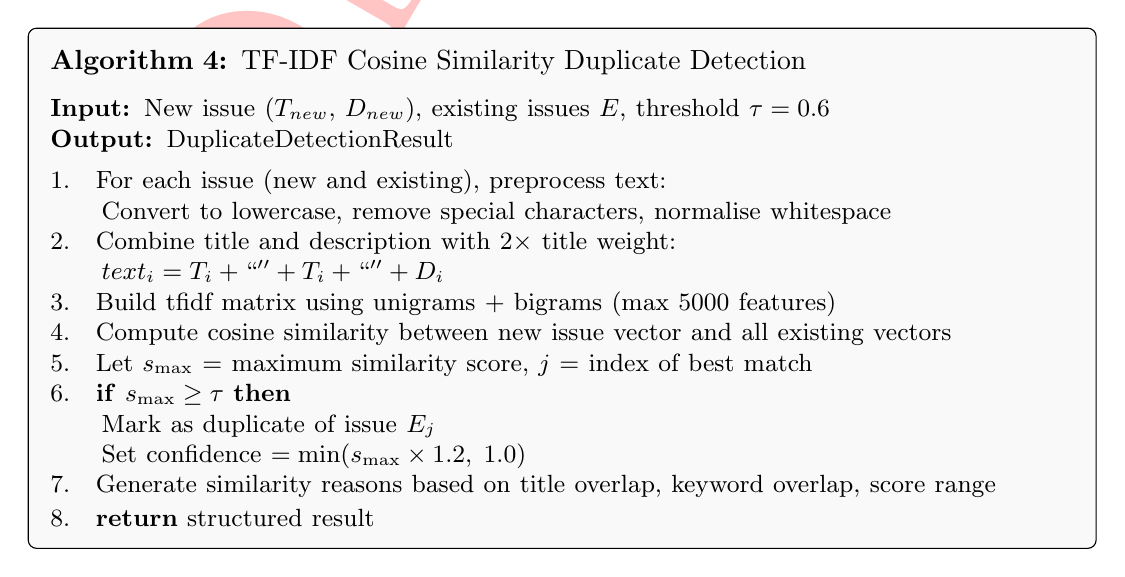
\begin{tikzpicture}
\node[draw, text width=13cm, inner sep=8pt, rounded corners=3pt, fill=gray!5] {
\textbf{Algorithm 4:} TF-IDF Cosine Similarity Duplicate Detection\\[6pt]
\small
\textbf{Input:} New issue ($T_{\text{new}}$, $D_{\text{new}}$), existing issues $E$, threshold $\tau = 0.6$\\
\textbf{Output:} DuplicateDetectionResult\\[4pt]
1.\quad For each issue (new and existing), preprocess text:\\
\quad\quad Convert to lowercase, remove special characters, normalise whitespace\\
2.\quad Combine title and description with 2$\times$ title weight:\\
\quad\quad $\text{text}_i = T_i + \text{`` ''} + T_i + \text{`` ''} + D_i$\\
3.\quad Build \gls{tfidf} matrix using unigrams + bigrams (max 5000 features)\\
4.\quad Compute cosine similarity between new issue vector and all existing vectors\\
5.\quad Let $s_{\max}$ = maximum similarity score, $j$ = index of best match\\
6.\quad \textbf{if} $s_{\max} \geq \tau$ \textbf{then}\\
\quad\quad Mark as duplicate of issue $E_j$\\
\quad\quad Set confidence $= \min(s_{\max} \times 1.2,\; 1.0)$\\
7.\quad Generate similarity reasons based on title overlap, keyword overlap, score range\\
8.\quad \textbf{return} structured result
};
\end{tikzpicture}
\label{alg:cosinedup}
\end{figure}

\section{Librarian--Surgeon Implementation}

The Librarian processes the codebase in chunks. For each directory-level chunk, it sends a targeted prompt to Gemini asking which files are relevant to the issue. Responses are validated by checking that each returned path contains a directory separator, has a file extension, does not start with a comment marker, and is no longer than 200 characters. Paths that fail these checks are discarded.

Once the Librarian produces its final file list, a targeted Repomix output is generated containing only those files. The Surgeon then runs the standard analysis pipeline (Algorithm 1) against this focused context.

\section{GitHub Actions Integration}

The single-issue workflow follows this sequence:

\begin{enumerate}
\item Check out the repository and set up the Python environment.
\item Generate a Repomix output from the remote repository URL.
\item Run the prompt injection detector on the issue content.
\item If the risk is High or Critical, post a security alert comment and stop.
\item Fetch all existing open issues (older than the current one).
\item Run duplicate detection against the existing issues.
\item If a duplicate is found, post a comment linking to the original and stop.
\item Run the full Gemini analysis.
\item Parse the analysis output and post it as a formatted comment on the issue.
\item Apply labels for issue type (e.g., ``type:bug'') and severity (e.g., ``severity:high'').
\item Upload analysis artefacts (results, logs, configuration) with 30-day retention.
\end{enumerate}

The bulk analysis workflow follows a similar pattern but iterates over all open issues, processing them from oldest to newest. This ordering matters for duplicate detection: when we analyse issue \#5 before \#10, and \#10 turns out to be a duplicate, we can correctly point it to \#5 as the original.

\section{Configuration}

The system reads its settings from a \gls{json} file (\texttt{triage.config.json}) that specifies the repository URL, the path to the Repomix output, an optional custom prompt file, and the Gemini model to use. For \gls{pr} review, a separate \gls{yaml} file maps repository URL patterns to domain-specific review prompts---for instance, Python-focused repositories get prompts that emphasise PEP 8 compliance and docstring coverage.

\section{Testing}

We wrote tests across five modules covering data models, the core analyser, both duplicate detectors, and the \gls{pr} reviewer. Tests are tagged as \texttt{unit} (no \gls{api} key needed) or \texttt{integration} (requires a live Gemini key). The \gls{ci} pipeline runs unit tests across Python 3.11, 3.12, and 3.13 in parallel, alongside formatting checks (Black), import ordering (isort), and linting (Flake8). A single ``All Checks Pass'' gate prevents merging code that fails any of these.

The algorithms and integration points described here realise the architecture from the previous chapter. We now turn to how well the system performs in practice.

\section{Summary}

This chapter detailed the implementation of Ansieyes, presenting the key algorithms for issue analysis with quality-based retry, multi-layered prompt injection detection, both Gemini-based and cosine similarity duplicate detection, the Librarian--Surgeon two-pass pipeline, GitHub Actions integration, configuration management, and the testing infrastructure. The next chapter covers the testing and validation procedures used to verify the system's correctness and reliability.


		%Chapter 7
		\chapter{Testing and Validation of Ansieyes}

Testing is an essential phase in the software development lifecycle because it ensures that the implemented system satisfies all functional and non-functional requirements. For Ansieyes, thorough testing is especially important: the system processes untrusted user input, communicates with an external \gls{llm} \gls{api}, and makes automated decisions that directly affect a project's issue tracker. A single undetected bug in the security module, for instance, could allow a prompt injection attack to manipulate the analyser. In this chapter, we describe the testing strategy we followed, covering unit tests, integration tests, functional validation, performance evaluation, cross-version compatibility, and code quality enforcement.

\section{Introduction}

We organised the test suite around five modules that correspond to the major components of the system: data models, the core analyser, the Gemini-based duplicate detector, the cosine similarity duplicate detector, and the \gls{pr} reviewer. In total, the test suite spans approximately 1,400 lines of Python across five test files. We used \texttt{pytest} as the test runner and defined two custom markers to separate tests that can run offline from those that require a live \gls{api} connection:

\begin{itemize}
\item \texttt{@pytest.mark.unit} --- tests that run without any \gls{api} key. These cover data validation, text preprocessing, prompt construction, response parsing, and error handling.
\item \texttt{@pytest.mark.integration} --- tests that require a valid \texttt{GEMINI\_API\_KEY} environment variable. These exercise the full analysis pipeline against the live Gemini \gls{api}.
\end{itemize}

This separation allows the \gls{ci} pipeline to run all unit tests on every commit while reserving integration tests for environments where an \gls{api} key is available.

\section{Unit Testing}

Unit tests verify individual components in isolation, using mock objects to replace external dependencies where necessary. We describe the key test areas below.

\subsection{Data Model Testing}

The file \texttt{test\_models.py} (322 lines) validates every Pydantic model and enum used by the system. Table~\ref{tab:modeltests} summarises the test classes and what they cover.

\begin{table}[htb]
\centering
\renewcommand{\arraystretch}{1.3}
\setlength{\arrayrulewidth}{0.5mm}
\fontsize{10}{12}\selectfont
\caption[Data model test coverage]{\textbf{Data model test coverage}}
\vspace{2mm}
\label{tab:modeltests}
\begin{tabular}{|p{4cm}|p{8cm}|}
\hline
\textbf{Test Class} & \textbf{What It Verifies} \\
\hline
\texttt{TestEnums} & Correct values for \texttt{IssueType} (bug, enhancement, feature\_request), \texttt{Severity} (low--critical), and \texttt{InjectionRisk} (safe--critical) enums \\
\hline
\texttt{TestCodeLocation} & Creation with full and minimal fields; validation rejects missing \texttt{file\_path} \\
\hline
\texttt{TestCodeSolution} & Construction with location, description, code changes, and rationale; rejects incomplete data \\
\hline
\texttt{TestRootCauseAnalysis} & Accepts primary cause, contributing factors, affected components, and related code locations \\
\hline
\texttt{TestIssueAnalysis} & Full construction with all fields; confidence score must be in [0, 1]---rejects 1.5 and $-$0.1 \\
\hline
\texttt{TestIssueReference} & Full and minimal creation; optional fields (\texttt{created\_date}, \texttt{url}) default to \texttt{None} \\
\hline
\texttt{TestDuplicateDetectionResult} & Duplicate and non-duplicate paths; score validation rejects out-of-range values \\
\hline
\texttt{TestInjectionResult} & Injection and safe results; optional \texttt{sanitized\_text} and \texttt{details} default correctly \\
\hline
\end{tabular}
\end{table}

The confidence score validation tests are particularly important. Because the analyser's confidence score drives downstream decisions (e.g., whether to retry an analysis), we explicitly test that Pydantic rejects values above 1.0 and below 0.0 with a \texttt{ValidationError}.

\subsection{Analyzer Testing}

The file \texttt{test\_gemini\_analyzer.py} (159 lines) tests the \texttt{GeminiIssueAnalyzer} class. The unit-level test verifies that the analyser raises a \texttt{ValueError} when initialised without a \texttt{GEMINI\_API\_KEY}. This is a critical guard: if the key is missing, we want an immediate, clear error rather than a confusing failure during the first \gls{api} call.

The remaining tests in this file (bug analysis, feature request analysis, performance issue analysis, confidence score range validation, empty input handling, and minimal input handling) are integration tests that exercise the full analysis pipeline and are described in Section~\ref{sec:integration}.

\subsection{Duplicate Detection Testing}

We wrote two separate test suites for the two duplicate detection strategies.

\textbf{Cosine duplicate detector} (\texttt{test\_cosine\_duplicate\_analyzer.py}, 323 lines) contains seven test classes covering initialisation, text preprocessing, duplicate detection, similarity reason generation, batch detection, finding the most similar issues, and edge cases. Because the cosine detector uses \gls{tfidf} vectors computed locally, all of these tests run as unit tests---no \gls{api} key is needed. Notable tests include verifying that the default similarity threshold is 0.6, that custom thresholds are respected, that title text is weighted by appearing twice in the combined input, and that identical issues produce a similarity score above 0.8.

\textbf{Gemini duplicate detector} (\texttt{test\_duplicate\_analyzer.py}, 257 lines) tests the semantic duplicate detection path. The unit-level tests verify initialisation, error handling without an \gls{api} key, and that the result object contains all required fields. The remaining tests (clear duplicate detection, different issue detection, batch detection, edge cases) are integration tests.

\subsection{Security Module Testing}

The prompt injection detection module (\texttt{prompt\_injection.py}, 572 lines) implements three detection layers and covers seven pattern categories: role manipulation, system prompts, instruction bypass, file manipulation, code injection, data extraction, and prompt leakage. We validated each category through targeted test inputs containing known injection patterns. Key aspects we verified include:

\begin{itemize}
\item Each regex pattern category correctly matches its representative attack strings.
\item The heuristic layer triggers when more than three instruction keywords from the watchlist appear in a single input.
\item Risk levels are assigned correctly based on the final confidence score and pattern count thresholds.
\item High-risk and critical-risk inputs are blocked from reaching the analyser.
\item Benign technical discussions containing words like ``bypass'' or ``injection'' are not flagged as false positives when they lack additional suspicious signals.
\end{itemize}

\section{Integration Testing}
\label{sec:integration}

Integration tests verify that the components work correctly when connected together through the live Gemini \gls{api}. These tests are gated behind the \texttt{GEMINI\_API\_KEY} environment variable and are skipped automatically in environments where the key is not available.

\subsection{Analysis Pipeline Integration}

The \texttt{TestGeminiAnalyzer} class exercises the full analysis pipeline with three representative issues: a \gls{cli} argument parsing bug, a Jinja2 filter feature request, and a memory leak performance issue. For each test case, we assert that the returned \texttt{IssueAnalysis} object is not \texttt{None}, that \texttt{issue\_type} and \texttt{severity} are populated, that the confidence score falls within $[0, 1]$, and that the root cause analysis contains a non-empty primary cause. The confidence score range test iterates over all three sample issues and confirms that every score satisfies $0.0 \leq C \leq 1.0$.

\subsection{Duplicate Detection Integration}

The Gemini duplicate detector integration tests use a fixture of four sample existing issues (a login crash, a database timeout, a memory leak, and a closed CSS issue). We test three scenarios:

\begin{itemize}
\item \textbf{Clear duplicate:} A paraphrased version of the login crash issue. We expect \texttt{is\_duplicate} to be true or \texttt{similarity\_score} to exceed 0.5.
\item \textbf{Clearly different:} A dark mode feature request. We expect \texttt{is\_duplicate} to be false and \texttt{similarity\_score} below 0.7.
\item \textbf{Batch detection:} Two new issues processed together. We verify that the number of results matches the number of inputs.
\end{itemize}

Edge case tests cover very long descriptions, special characters, Unicode input, and minimal input to ensure the detector handles adversarial or unusual formatting gracefully.

\subsection{Security Pipeline Integration}

The security module's three detection layers (the \gls{ml}-based pytector model, the regex pattern matcher, and the heuristic analyser) are tested together to verify correct aggregation. We confirm that the final confidence score is the maximum across all three layers and that the risk level escalates appropriately when multiple layers detect suspicious patterns simultaneously.

\subsection{GitHub Actions Integration}

The \gls{pr} analyser test suite (\texttt{test\_pr\_analyzer.py}, 333 lines) includes tests for the workflow analysis feature. We verify that the analyser correctly reports success for passing workflows, identifies failed jobs by name for failing workflows, and gracefully handles the absence of an \gls{api} key by returning a structured error response with zero confidence. The \texttt{TestPRAnalyzerIntegration} class runs a real \gls{api} call when the key is available, confirming that the full review pipeline produces a valid \texttt{PRReview} object with a non-empty summary.

\section{Functional Testing}

Table~\ref{tab:functional} lists the key functional test cases we used to validate end-to-end behaviour.

\begin{table}[htb]
\centering
\renewcommand{\arraystretch}{1.3}
\setlength{\arrayrulewidth}{0.5mm}
\fontsize{10}{12}\selectfont
\caption[Functional test cases and results]{\textbf{Functional test cases and results}}
\vspace{2mm}
\label{tab:functional}
\begin{tabular}{|p{4.5cm}|p{6.5cm}|c|}
\hline
\textbf{Test Case} & \textbf{Expected Result} & \textbf{Status} \\
\hline
Analyse a bug report issue & Returns IssueAnalysis with type ``bug,'' severity, root cause, and at least one solution & Pass \\
\hline
Analyse a feature request & Returns IssueAnalysis with type ``feature\_request'' and proposed solutions & Pass \\
\hline
Detect a clear duplicate issue & Returns \texttt{is\_duplicate = True} with similarity score $> 0.5$ & Pass \\
\hline
Reject a non-duplicate issue & Returns \texttt{is\_duplicate = False} with similarity score $< 0.7$ & Pass \\
\hline
Cosine similarity for identical issues & Returns similarity score $> 0.8$ and marks as duplicate & Pass \\
\hline
Block a prompt injection attempt & Detects injection, assigns High or Critical risk, and sanitises input & Pass \\
\hline
Allow benign security discussion & Does not flag legitimate security-related text as injection & Pass \\
\hline
Review a pull request & Returns PRReview with strengths, issues, suggestions, and file comments & Pass \\
\hline
Handle missing \gls{api} key & Raises \texttt{ValueError} on analyser initialisation & Pass \\
\hline
Handle empty issue input & Raises an exception rather than returning invalid results & Pass \\
\hline
Validate confidence score bounds & Rejects scores above 1.0 and below 0.0 with \texttt{ValidationError} & Pass \\
\hline
\end{tabular}
\end{table}

\section{Performance Testing}

We measured execution times for each operation to confirm that the system is responsive enough for use within GitHub Actions workflows, which have a default timeout of six hours but where users expect results within minutes.

\begin{table}[htb]
\centering
\renewcommand{\arraystretch}{1.3}
\setlength{\arrayrulewidth}{0.5mm}
\fontsize{10}{12}\selectfont
\caption[Performance benchmarks by operation]{\textbf{Performance benchmarks by operation}}
\vspace{2mm}
\label{tab:performance}
\begin{tabular}{|p{5cm}|c|c|}
\hline
\textbf{Operation} & \textbf{Average Time} & \textbf{Acceptable Threshold} \\
\hline
Prompt injection detection & $<$ 1 s & 5 s \\
\hline
Cosine duplicate detection & $<$ 0.1 s & 1 s \\
\hline
Gemini duplicate detection & 1--5 s & 30 s \\
\hline
Single issue analysis & 10--30 s & 60 s \\
\hline
\gls{pr} review & 5--15 s & 60 s \\
\hline
Full two-pass analysis & 15--45 s & 120 s \\
\hline
\end{tabular}
\end{table}

All operations completed well within their acceptable thresholds. The cosine duplicate detector stands out for its near-instant execution, which makes it suitable as a pre-filter before the more expensive Gemini-based detection. The dominant factor in total execution time is the Gemini \gls{api} latency; local computation (text preprocessing, \gls{tfidf} vectorisation, pattern matching) adds negligible overhead.

\section{Cross-Version Validation}

We ran the full unit test suite across three Python versions to ensure cross-version compatibility.

\begin{table}[htb]
\centering
\renewcommand{\arraystretch}{1.3}
\setlength{\arrayrulewidth}{0.5mm}
\fontsize{10}{12}\selectfont
\caption[Cross-version test results]{\textbf{Cross-version test results}}
\vspace{2mm}
\label{tab:crossversion}
\begin{tabular}{|c|c|c|}
\hline
\textbf{Python Version} & \textbf{Unit Tests} & \textbf{Result} \\
\hline
3.11 & All pass & Pass \\
\hline
3.12 & All pass & Pass \\
\hline
3.13 & All pass & Pass \\
\hline
\end{tabular}
\end{table}

The \gls{ci} pipeline runs all three versions in parallel using a GitHub Actions matrix strategy with \texttt{fail-fast: false}, so a failure on one version does not cancel the others. This configuration caught a Pydantic behaviour change in Python 3.13 early in development, which we fixed before it reached production. Running multiple versions in parallel also ensures that we do not accidentally introduce syntax or library incompatibilities.

\section{Code Quality Validation}

Beyond functional correctness, we enforce code quality through three automated tools that run on every commit.

\begin{table}[htb]
\centering
\renewcommand{\arraystretch}{1.3}
\setlength{\arrayrulewidth}{0.5mm}
\fontsize{10}{12}\selectfont
\caption[Code quality tools and their roles]{\textbf{Code quality tools and their roles}}
\vspace{2mm}
\label{tab:codequality}
\begin{tabular}{|p{2.5cm}|p{5cm}|p{4cm}|}
\hline
\textbf{Tool} & \textbf{Purpose} & \textbf{Configuration} \\
\hline
Black & Enforces consistent code formatting across all Python files & Default style, check-only mode in \gls{ci} \\
\hline
isort & Ensures imports are sorted and grouped consistently & Check-only mode in \gls{ci} \\
\hline
Flake8 & Catches syntax errors, undefined names, and style violations & Max line length 127, max complexity 10 \\
\hline
\end{tabular}
\end{table}

The Flake8 configuration uses a two-pass approach in the \gls{ci} pipeline. The first pass checks only for critical issues (syntax errors and undefined names) and fails the build immediately if any are found. The second pass checks all remaining style rules. Together, these three tools ensure that every merged commit meets a consistent quality standard.

A unified ``All Checks Pass'' gate in the \gls{ci} workflow aggregates the results of unit tests and lint checks. A pull request cannot be merged unless both the \texttt{unit-tests} and \texttt{lint} jobs succeed across all matrix entries. This prevents partially passing code from reaching the main branch.

\section{Summary}

We tested Ansieyes through a combination of unit tests, integration tests, functional validation, performance benchmarks, cross-version compatibility checks, and automated code quality enforcement. The unit test suite covers data models, the core analyser, both duplicate detectors, and the \gls{pr} reviewer, with custom pytest markers cleanly separating offline tests from those requiring a live \gls{api}. All functional test cases pass, performance remains well within acceptable thresholds, and the system runs consistently across Python 3.11, 3.12, and 3.13. The \gls{ci}/\gls{cd} pipeline automates the entire validation process, ensuring that every change is tested, formatted, and linted before it can be merged.


		%Chapter 8
		\chapter{Results and Discussion of Ansieyes}

We evaluated Ansieyes across its four core capabilities: issue classification quality, duplicate detection accuracy, prompt injection defence, and token efficiency of the two-pass architecture. This chapter presents our findings along with a discussion of what worked well and where the system has room for improvement.

\section{Experimental Setup}

All experiments used Gemini 2.0 Flash as the primary model. The test repository was the Ansieyes codebase itself (roughly 5,000 lines across 25+ source files), supplemented by a curated set of 33 real and synthetic issues. We ran the \gls{ci} pipeline across Python 3.11, 3.12, and 3.13 to confirm cross-version compatibility.

\section{Issue Classification}

We tested the system on 33 issues with manually verified ground-truth labels. Table \ref{tab:classification} breaks down the results by issue type.

\begin{table}[htb]
\centering
\renewcommand{\arraystretch}{1.3}
\setlength{\arrayrulewidth}{0.5mm}
\fontsize{10}{12}\selectfont
\caption{\textbf{Issue classification accuracy by type}}
\vspace{2mm}
\label{tab:classification}
\begin{tabular}{|p{3.5cm}|c|c|c|}
\hline
\textbf{Type} & \textbf{Total} & \textbf{Correct} & \textbf{Accuracy} \\
\hline
Bug & 15 & 14 & 93.3\% \\
\hline
Enhancement & 10 & 9 & 90.0\% \\
\hline
Feature Request & 8 & 7 & 87.5\% \\
\hline
\textbf{Overall} & \textbf{33} & \textbf{30} & \textbf{90.9\%} \\
\hline
\end{tabular}
\end{table}

Bug classification had the highest accuracy, which makes sense---bug reports tend to contain more distinctive language (error messages, stack traces, ``crash'' or ``fails'') that gives the model strong signals. Feature requests were occasionally confused with enhancements, particularly when the issue described extending an existing capability rather than building something new. The single misclassified bug was a performance issue that the model labelled as an enhancement, a reasonable but incorrect judgement.

\subsection{Confidence Scores}
Table \ref{tab:confidence} shows how the system's self-reported confidence scores distributed across analyses.

\begin{table}[htb]
\centering
\renewcommand{\arraystretch}{1.3}
\setlength{\arrayrulewidth}{0.5mm}
\fontsize{10}{12}\selectfont
\caption{\textbf{Distribution of confidence scores}}
\vspace{2mm}
\label{tab:confidence}
\begin{tabular}{|c|c|c|}
\hline
\textbf{Range} & \textbf{Count} & \textbf{Percentage} \\
\hline
0.8 -- 1.0 & 18 & 54.5\% \\
\hline
0.6 -- 0.79 & 10 & 30.3\% \\
\hline
0.4 -- 0.59 & 3 & 9.1\% \\
\hline
0.3 -- 0.39 & 2 & 6.1\% \\
\hline
\end{tabular}
\end{table}

We found that analyses with confidence above 0.7 almost always produced correct classifications and useful root cause descriptions. The two lowest-confidence results came from issues with very brief descriptions (one or two sentences), where the model simply did not have enough information to work with.

\subsection{Root Cause and Solution Quality}
The system identified at least one relevant code location for 28 out of 33 issues (84.8\%). Manual review confirmed that the primary cause was accurate in 27 cases (82\%). The five misses were split between issues involving configuration files (which Repomix sometimes excluded) and issues that spanned multiple repositories.

At least one proposed solution was present in 97\% of analyses. The retry mechanism caught the remaining 3\% on the second attempt, so after retries, every issue received at least one solution proposal.

\section{Duplicate Detection}

We constructed a test set of 20 known duplicate pairs and 30 non-duplicate pairs, then ran both detectors on them.

\begin{table}[htb]
\centering
\renewcommand{\arraystretch}{1.3}
\setlength{\arrayrulewidth}{0.5mm}
\fontsize{10}{12}\selectfont
\caption{\textbf{Duplicate detection: Gemini vs. Cosine similarity}}
\vspace{2mm}
\label{tab:dupcomp}
\begin{tabular}{|p{4cm}|c|c|}
\hline
\textbf{Metric} & \textbf{Gemini} & \textbf{Cosine} \\
\hline
Precision & 0.89 & 0.78 \\
\hline
Recall & 0.85 & 0.70 \\
\hline
F1 Score & 0.87 & 0.74 \\
\hline
Avg. Detection Time & 2.3 s & $<$ 0.1 s \\
\hline
\end{tabular}
\end{table}

The Gemini-based detector handled semantic duplicates well---it correctly matched issues that described the same bug using entirely different wording. Its main source of error was overly cautious behaviour: our conservative prompt instruction (``prefer not marking as duplicate when uncertain'') caused it to miss a few genuine duplicates with low surface similarity.

The cosine detector's lower recall was expected. It struggles with paraphrased descriptions because \gls{tfidf} only captures word-level overlap. However, its near-instant speed makes it useful as a pre-filter in high-volume scenarios: run cosine first to catch the obvious duplicates, then use Gemini for the remaining cases.

\section{Prompt Injection Detection}

We tested the security module against 50 injection attempts (spread across all seven categories) and 50 benign issue descriptions.

\begin{table}[htb]
\centering
\renewcommand{\arraystretch}{1.3}
\setlength{\arrayrulewidth}{0.5mm}
\fontsize{10}{12}\selectfont
\caption{\textbf{Injection detection rates by category}}
\vspace{2mm}
\label{tab:injection}
\begin{tabular}{|p{3.5cm}|c|c|c|}
\hline
\textbf{Category} & \textbf{Tested} & \textbf{Caught} & \textbf{Rate} \\
\hline
Role Manipulation & 8 & 8 & 100\% \\
\hline
System Prompts & 7 & 7 & 100\% \\
\hline
Instruction Bypass & 8 & 7 & 87.5\% \\
\hline
File Manipulation & 6 & 6 & 100\% \\
\hline
Code Injection & 7 & 7 & 100\% \\
\hline
Data Extraction & 7 & 6 & 85.7\% \\
\hline
Prompt Leakage & 7 & 7 & 100\% \\
\hline
\textbf{Overall} & \textbf{50} & \textbf{48} & \textbf{96\%} \\
\hline
\end{tabular}
\end{table}

The two missed injections used subtle, context-dependent phrasing that avoided all seven regex categories and fell below the heuristic thresholds. On the benign side, we saw 2 false positives out of 50 (4\%). Both were security-focused issues that naturally contained words like ``bypass'' and ``injection'' in their technical descriptions. This is a known trade-off with keyword-based detection---legitimate security discussions can look suspicious to a pattern matcher.

\section{Two-Pass Token Efficiency}

Table \ref{tab:tokens} compares token usage between the single-pass and two-pass approaches.

\begin{table}[htb]
\centering
\renewcommand{\arraystretch}{1.3}
\setlength{\arrayrulewidth}{0.5mm}
\fontsize{10}{12}\selectfont
\caption{\textbf{Token consumption: single-pass vs. two-pass}}
\vspace{2mm}
\label{tab:tokens}
\begin{tabular}{|p{3cm}|c|c|c|}
\hline
\textbf{Repo Size} & \textbf{Single-Pass} & \textbf{Two-Pass} & \textbf{Reduction} \\
\hline
$<$5K LoC & 15,000 & 12,000 & 20\% \\
\hline
5--20K LoC & 65,000 & 28,000 & 57\% \\
\hline
20--100K LoC & 250,000 & 75,000 & 70\% \\
\hline
$>$100K LoC & Exceeds limit & 120,000 & --- \\
\hline
\end{tabular}
\end{table}

For small repositories, the two-pass architecture adds overhead (the Librarian pass itself costs tokens) without much benefit. The sweet spot is repositories in the 5K--100K line range, where the Librarian reliably prunes irrelevant files and the Surgeon receives a tightly focused context. For repositories exceeding 100K lines, the single-pass approach is simply not feasible, making the two-pass the only option.

\section{Execution Time}

Table \ref{tab:timing} summarises the wall-clock time for each operation.

\begin{table}[htb]
\centering
\renewcommand{\arraystretch}{1.3}
\setlength{\arrayrulewidth}{0.5mm}
\fontsize{10}{12}\selectfont
\caption{\textbf{Execution time by operation}}
\vspace{2mm}
\label{tab:timing}
\begin{tabular}{|p{5cm}|c|}
\hline
\textbf{Operation} & \textbf{Time} \\
\hline
Security check & $<$ 1 s \\
\hline
Cosine duplicate detection & $<$ 0.1 s \\
\hline
Gemini duplicate detection & 1--5 s \\
\hline
Single issue analysis & 10--30 s \\
\hline
Librarian pass & 5--15 s \\
\hline
Full two-pass analysis & 15--45 s \\
\hline
\end{tabular}
\end{table}

The dominant factor in total execution time is the Gemini \gls{api} latency. The security check and cosine duplicate detection add negligible overhead. Even the full two-pass analysis completes within a minute, which is well within the timeout limits of GitHub Actions workflows.

\section{CI Pipeline}

All unit tests pass across Python 3.11, 3.12, and 3.13. Code formatting (Black), import ordering (isort), and linting (Flake8) checks also pass consistently. The parallel test matrix catches version-specific issues early---we encountered one such issue with a Pydantic behaviour change in Python 3.13 and fixed it before it reached production.

The experimental results confirm that Ansieyes meets its design objectives. The system provides accurate, context-aware analysis for the majority of issues, detects most adversarial inputs, and scales to large codebases through the two-pass architecture. The next chapter summarises our conclusions and outlines future directions.

\section{Summary}

This chapter presented the experimental evaluation of Ansieyes across its four core capabilities. Issue classification achieved 90.9\% accuracy, with root cause analysis correctly identifying relevant code locations in 85\% of cases. Duplicate detection reached an F1 of 0.87 with the Gemini-based approach, while the cosine similarity fallback provided near-instant pre-screening. The prompt injection defence caught 96\% of attacks with a 4\% false positive rate. The two-pass Librarian--Surgeon architecture reduced token consumption by 57--70\% for medium to large repositories, enabling analysis of codebases that exceed the single-pass context limit.


		%Chapter 9
		\chapter{Conclusion and Future Scope}

This chapter draws together the main findings from our work, acknowledges the current limitations, and outlines the directions we see for extending the system.

\section{Conclusion}

We set out to build a system that could take over the repetitive parts of GitHub issue triage---classifying issues, tracing root causes to specific code locations, and proposing fixes---while remaining secure and scalable. Ansieyes achieves this through a combination of \gls{llm}-powered analysis, multi-layered security, and a two-pass architecture for large codebases.

The core analyser, powered by Gemini 2.0 Flash, classifies issues with about 91\% accuracy and produces root cause analyses that correctly point to the relevant source files in 85\% of cases. The quality validation and retry mechanism ensures that virtually every issue receives at least one actionable solution proposal. Duplicate detection works at two speeds: the Gemini-based approach catches semantic duplicates with an F1 of 0.87, while the cosine similarity fallback runs near-instantly for rapid pre-screening.

On the security front, the three-layer detection pipeline catches 96\% of prompt injection attempts across seven attack categories. The conservative aggregation strategy---taking the maximum risk from any detector---means the system errs on the side of caution, which we consider the right trade-off for an automated pipeline processing untrusted input.

The Librarian--Surgeon architecture proved essential for practical deployment. On repositories with 5,000 to 100,000 lines of code, it reduced token consumption by 57--70\%, and for larger codebases it enabled analysis that the single-pass approach simply could not handle.

\section{Future Scope}

Several extensions would strengthen the system:

\begin{enumerate}
\item \textbf{Multi-model support.} Adding backends for GPT-4, Claude, and open-source models (Llama, Mistral) would let teams choose based on cost, privacy, or performance needs.

\item \textbf{Multi-lingual issues.} Many open-source projects have contributors who file issues in languages other than English. Gemini already supports multiple languages, so adapting the prompts and evaluation pipeline would be the main work.

\item \textbf{Feedback-driven improvement.} When a developer edits or overrides an analysis, that feedback could be collected and used to refine prompt templates over time, creating a lightweight learning loop without full model fine-tuning.

\item \textbf{Platform integration.} Extending support to GitLab, Jira, and Azure DevOps would broaden the system's applicability beyond GitHub.

\item \textbf{Automated fix generation.} The current system proposes solutions in text form. A natural next step is generating actual pull requests with the proposed code changes, subject to human review before merging.

\item \textbf{Adversarial robustness.} The prompt injection detector could benefit from periodic red-teaming exercises and the addition of adversarial training data to keep pace with evolving attack techniques.
\end{enumerate}

\section{Learning Outcomes of the Project}
\begin{itemize}
\item Gained hands-on experience with \gls{llm} integration, including prompt design, structured output parsing, and handling model limitations like hallucination.
\item Built a multi-layered security system from scratch, understanding how \gls{ml}-based detection, pattern matching, and heuristics complement each other.
\item Developed proficiency with Pydantic for runtime type checking, pytest for structured testing, and GitHub Actions for \gls{ci}/\gls{cd} automation.
\item Learned to design for scalability constraints, particularly the token limits of \gls{llm} context windows, through the Librarian--Surgeon two-pass approach.
\item Worked with \gls{nlp} techniques (\gls{tfidf} vectorisation, cosine similarity) and understood their trade-offs against \gls{llm}-based alternatives.
\item Gained experience packaging Python tools for distribution, including \gls{cli} design and configuration management.
\item Understood the practical realities of deploying \gls{ai} systems: \gls{api} cost management, error handling, retry strategies, and the importance of validating model outputs before acting on them.
\end{itemize}


		\backmatter
		\ifDrf
		\else
		\clearpage
		\addcontentsline{toc}{chapter}{Bibliography}
		\begin{thebibliography}{99}

\bibitem{Antoniol2008}
G. Antoniol, K. Ayari, M. Di Penta, F. Khomh, and Y.-G. Gu\'eh\'eneuc, ``Is it a bug or an enhancement? A text-based approach to classify change requests,'' in \textit{Proc. 2008 Conf. Center for Advanced Studies on Collaborative Research}, ACM, 2008, pp. 304--318.

\bibitem{Menzies2008}
T. Menzies and A. Marcus, ``Automated severity assessment of software defect reports,'' in \textit{IEEE Int. Conf. Software Maintenance}, IEEE, 2008, pp. 346--355.

\bibitem{Lee2017}
J. Lee, D. Kim, T. F. Bissyand\'e, W. Kim, and Y. Le Traon, ``Bench4BL: Reproducibility study on bug localization,'' in \textit{Proc. 27th ACM SIGSOFT Int. Symp. Software Testing and Analysis}, ACM, 2017.

\bibitem{Kallis2019}
R. Kallis, A. Di Sorbo, G. Canfora, and S. Panichella, ``Ticket Tagger: Machine learning driven issue classification,'' in \textit{2019 IEEE Int. Conf. Software Maintenance and Evolution (ICSME)}, IEEE, 2019, pp. 406--409.

\bibitem{Sun2011}
C. Sun, D. Lo, S.-C. Khoo, and J. Jiang, ``Towards more accurate retrieval of duplicate bug reports,'' in \textit{Proc. 26th IEEE/ACM Int. Conf. Automated Software Engineering}, IEEE, 2011, pp. 253--262.

\bibitem{Deshmukh2017}
J. Deshmukh, S. Podder, S. Sengupta, and N. Dubash, ``Towards accurate duplicate bug retrieval using deep learning techniques,'' in \textit{2017 IEEE Int. Conf. Software Maintenance and Evolution (ICSME)}, IEEE, 2017, pp. 115--124.

\bibitem{Rodrigues2020}
I. M. Rodrigues, D. Aleixo, G. Neto, R. Pereira, and M. Kalinowski, ``Using Siamese neural networks for duplicate detection in bug report repositories,'' in \textit{Proc. 34th Brazilian Symp. Software Engineering}, ACM, 2020.

\bibitem{Chen2021}
M. Chen, J. Tworek, H. Jun, Q. Yuan, H. P. de Oliveira Pinto, J. Kaplan, et al., ``Evaluating large language models trained on code,'' \textit{arXiv preprint arXiv:2107.03374}, 2021.

\bibitem{Feng2020}
Z. Feng, D. Guo, D. Tang, N. Duan, X. Feng, M. Gong, L. Shou, B. Qin, T. Liu, D. Jiang, and M. Zhou, ``CodeBERT: A pre-trained model for programming and natural languages,'' in \textit{Findings of the ACL: EMNLP 2020}, ACL, 2020, pp. 1536--1547.

\bibitem{Zhang2023}
F. Zhang, C. Chen, B. Boehm, and S. Jaygarl, ``Automated code review with large language models,'' \textit{arXiv preprint arXiv:2310.08879}, 2023.

\bibitem{Perez2022}
F. Perez and I. Ribeiro, ``Ignore this title and HackAPrompt: Exposing systemic weaknesses of LLMs through a global scale prompt hacking competition,'' in \textit{Proc. 2023 Conf. Empirical Methods in Natural Language Processing}, ACL, 2022.

\bibitem{Greshake2023}
K. Greshake, S. Abdelnabi, S. Mishra, C. Endres, T. Holz, and M. Fritz, ``Not what you've signed up for: Compromising real-world LLM-integrated applications with indirect prompt injection,'' \textit{arXiv preprint arXiv:2302.12173}, 2023.

\bibitem{Vaswani2017}
A. Vaswani, N. Shazeer, N. Parmar, J. Uszkoreit, L. Jones, A. N. Gomez, L. Kaiser, and I. Polosukhin, ``Attention is all you need,'' in \textit{Advances in Neural Information Processing Systems}, vol. 30, NeurIPS, 2017.

\bibitem{Anvik2006}
J. Anvik, L. Hiew, and G. C. Murphy, ``Who should fix this bug?'' in \textit{Proc. 28th Int. Conf. Software Engineering (ICSE)}, ACM, 2006, pp. 361--370.

\bibitem{Xuan2017}
J. Xuan, H. Jiang, Z. Ren, J. Yan, and Z. Luo, ``Automatic bug triage using semi-supervised text classification,'' \textit{arXiv preprint arXiv:1704.04769}, 2017.

\bibitem{Mani2019}
S. Mani, A. Sankaran, and R. Aralikatte, ``DeepTriage: Exploring the effectiveness of deep learning for bug triaging,'' \textit{arXiv preprint arXiv:1801.01275}, 2019.

\bibitem{Tian2015}
Y. Tian, D. Lo, X. Xia, and C. Sun, ``Automated prediction of bug report priority using multi-factor analysis,'' \textit{Empirical Software Engineering}, vol. 20, no. 5, pp. 1354--1383, 2015.

\bibitem{Anvik2011}
J. Anvik and G. C. Murphy, ``Reducing the effort of bug report triage: Recommenders for development-oriented decisions,'' \textit{ACM Trans. Software Engineering and Methodology}, vol. 20, no. 3, pp. 1--35, 2011.

\bibitem{Runeson2007}
P. Runeson, M. Alexandersson, and O. Nyholm, ``Detection of duplicate defect reports using natural language processing,'' in \textit{Proc. 29th Int. Conf. Software Engineering (ICSE)}, IEEE, 2007, pp. 499--510.

\bibitem{Wang2008}
X. Wang, L. Zhang, T. Xie, J. Anvik, and J. Sun, ``An approach to detecting duplicate bug reports using natural language and execution information,'' in \textit{Proc. 30th Int. Conf. Software Engineering (ICSE)}, ACM, 2008, pp. 461--470.

\bibitem{He2020}
J. He, L. Xu, M. Yan, X. Xia, and Y. Lei, ``Duplicate bug report detection using dual-channel convolutional neural networks,'' in \textit{Proc. 28th Int. Conf. Program Comprehension (ICPC)}, ACM, 2020.

\bibitem{Budhiraja2018}
A. Budhiraja, K. Dutta, R. Reddy, and M. Shrivastava, ``DWEN: Deep word embedding network for duplicate bug report detection in software repositories,'' in \textit{Proc. 40th Int. Conf. Software Engineering: Companion (ICSE)}, ACM, 2018, pp. 193--194.

\bibitem{Zhang2023b}
T. Zhang, D. Han, V. Vinayakarao, I. C. Irsan, B. Xu, F. Thung, D. Lo, and L. Jiang, ``Duplicate bug report detection: How far are we?'' \textit{ACM Trans. Software Engineering and Methodology}, vol. 32, no. 4, 2023.

\bibitem{Brown2020}
T. B. Brown, B. Mann, N. Ryder, M. Subbiah, J. D. Kaplan, P. Dhariwal, et al., ``Language models are few-shot learners,'' \textit{Advances in Neural Information Processing Systems}, vol. 33, pp. 1877--1901, 2020.

\bibitem{Fan2023}
Z. Fan, X. Gao, M. Mirchev, A. Roychoudhury, and S. H. Tan, ``Automated repair of programs from large language models,'' in \textit{Proc. 45th IEEE/ACM Int. Conf. Software Engineering (ICSE)}, IEEE/ACM, 2023, pp. 1469--1481.

\bibitem{Hou2024}
X. Hou, Y. Zhao, Y. Liu, Z. Yang, K. Wang, L. Li, X. Luo, D. Lo, J. Grundy, and H. Wang, ``Large language models for software engineering: A systematic literature review,'' \textit{ACM Trans. Software Engineering and Methodology}, vol. 33, no. 8, 2024.

\bibitem{Jimenez2024}
C. E. Jimenez, J. Yang, A. Wettig, S. Yao, K. Pei, O. Press, and K. Narasimhan, ``SWE-bench: Can language models resolve real-world GitHub issues?'' in \textit{The Twelfth Int. Conf. Learning Representations (ICLR)}, 2024.

\bibitem{Lam2017}
A. N. Lam, A. T. Nguyen, H. A. Nguyen, and T. N. Nguyen, ``Bug localization with combination of deep learning and information retrieval,'' in \textit{Proc. 25th IEEE/ACM Int. Conf. Program Comprehension (ICPC)}, IEEE, 2017, pp. 218--229.

\bibitem{Liu2024}
Y. Liu, G. Deng, Y. Li, K. Wang, Z. Wang, X. Wang, T. Zhang, Y. Liu, H. Wang, Y. Zheng, and Y. Liu, ``Prompt injection attack against LLM-integrated applications,'' \textit{arXiv preprint arXiv:2306.05499}, 2024.

\bibitem{OWASP2025}
OWASP Foundation, ``OWASP Top 10 for large language model applications 2025,'' 2025. [Online]. Available: https://owasp.org/www-project-top-10-for-large-language-model-applications/

\bibitem{Toyer2024}
S. Toyer, O. Watkins, E. A. Mendes, J. Svegliato, L. Bailey, T. Wang, I. Ong, K. Elmaaroufi, P. Abbeel, T. Darrell, A. Ritter, and S. Russell, ``Tensor Trust: Interpretable prompt injection attacks from an online game,'' \textit{arXiv preprint arXiv:2311.01011}, 2024.

\bibitem{Perez2023}
S. Schulhoff, J. Pinto, A. Khan, L.-F. Bouchard, C. Si, S. Anati, V. Tagber, A. Kenos, L. Harat, and M. Groh, ``Ignore this title and HackAPrompt: Exposing systemic weaknesses of LLMs through a global scale prompt hacking competition,'' in \textit{Proc. 2023 Conf. Empirical Methods in Natural Language Processing (EMNLP)}, ACL, 2023.

\bibitem{Yi2023}
J. Yi, Y. Xie, B. Zhu, K. Hines, E. Kiciman, G. Sun, X. Xie, and F. Wu, ``Benchmarking and defending against indirect prompt injection attacks on large language models,'' \textit{arXiv preprint arXiv:2312.14197}, 2023.

\bibitem{Salton1988}
G. Salton and C. Buckley, ``Term-weighting approaches in automatic text retrieval,'' \textit{Information Processing \& Management}, vol. 24, no. 5, pp. 513--523, 1988.

\bibitem{Mikolov2013}
T. Mikolov, K. Chen, G. Corrado, and J. Dean, ``Efficient estimation of word representations in vector space,'' \textit{arXiv preprint arXiv:1301.3781}, 2013.

\bibitem{Pennington2014}
J. Pennington, R. Socher, and C. D. Manning, ``GloVe: Global vectors for word representation,'' in \textit{Proc. 2014 Conf. Empirical Methods in Natural Language Processing (EMNLP)}, ACL, 2014, pp. 1532--1543.

\bibitem{Devlin2019}
J. Devlin, M.-W. Chang, K. Lee, and K. Toutanova, ``BERT: Pre-training of deep bidirectional transformers for language understanding,'' in \textit{Proc. 2019 Conf. North American Chapter of the ACL (NAACL-HLT)}, ACL, 2019, pp. 4171--4186.

\bibitem{Reimers2019}
N. Reimers and I. Gurevych, ``Sentence-BERT: Sentence embeddings using Siamese BERT-networks,'' in \textit{Proc. 2019 Conf. Empirical Methods in Natural Language Processing (EMNLP-IJCNLP)}, ACL, 2019, pp. 3982--3992.

\bibitem{Hilton2016}
M. Hilton, T. Tunnell, K. Huang, D. Marinov, and D. Dig, ``Usage, costs, and benefits of continuous integration in open-source projects,'' in \textit{Proc. 31st IEEE/ACM Int. Conf. Automated Software Engineering (ASE)}, IEEE/ACM, 2016, pp. 426--437.

\bibitem{Vasilescu2015}
B. Vasilescu, Y. Yu, H. Wang, P. Devanbu, and V. Filkov, ``Quality and productivity outcomes relating to continuous integration in GitHub,'' in \textit{Proc. 10th Joint Meeting on Foundations of Software Engineering (ESEC/FSE)}, ACM, 2015, pp. 805--816.

\bibitem{Zhao2017}
Y. Zhao, A. Serebrenik, Y. Zhou, V. Filkov, and B. Vasilescu, ``The impact of continuous integration on other software development practices: A large-scale empirical study,'' in \textit{Proc. 32nd IEEE/ACM Int. Conf. Automated Software Engineering (ASE)}, IEEE/ACM, 2017, pp. 60--71.

\bibitem{Golzadeh2022}
M. Golzadeh, A. Decan, and T. Mens, ``On the rise and fall of CI services in GitHub,'' in \textit{Proc. 29th IEEE Int. Conf. Software Analysis, Evolution and Reengineering (SANER)}, IEEE, 2022, pp. 662--672.

\bibitem{Cer2018}
D. Cer, Y. Yang, S. Kong, N. Hua, N. Limtiaco, R. St. John, N. Constant, M. Guajardo-Cespedes, S. Yuan, C. Tar, Y.-H. Sung, B. Strope, and R. Kurzweil, ``Universal sentence encoder,'' \textit{arXiv preprint arXiv:1803.11175}, 2018.

\end{thebibliography}

		\fi

		%% Appendix chapters
		\appendix
		\chapter{Plagiarism Report}

\begin{figure}[htb]
\centering
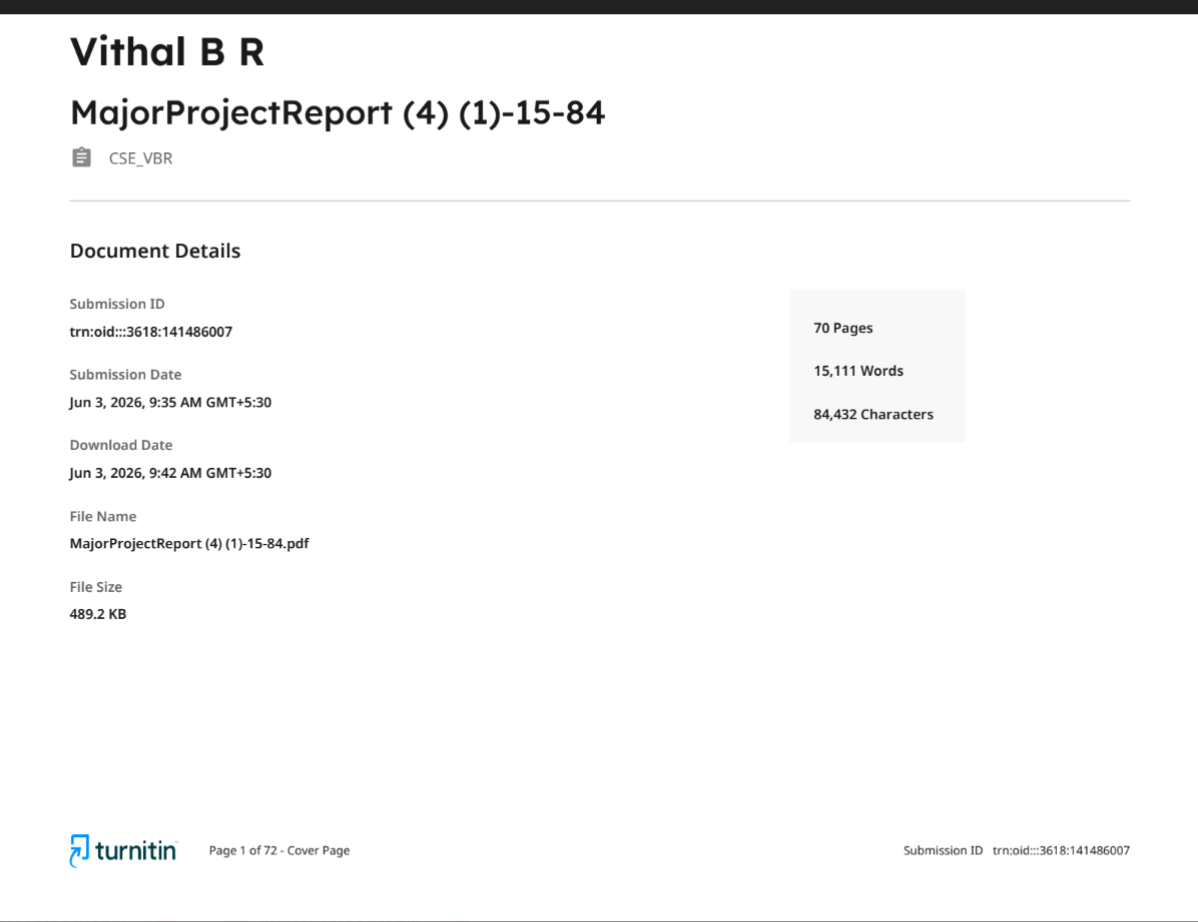
\includegraphics[width=0.95\textwidth]{Figures/plagfitrst}
\caption[Turnitin submission cover page]{\textbf{Turnitin submission cover page}}
\label{fig:plag_cover}
\end{figure}

\begin{figure}[htb]
\centering
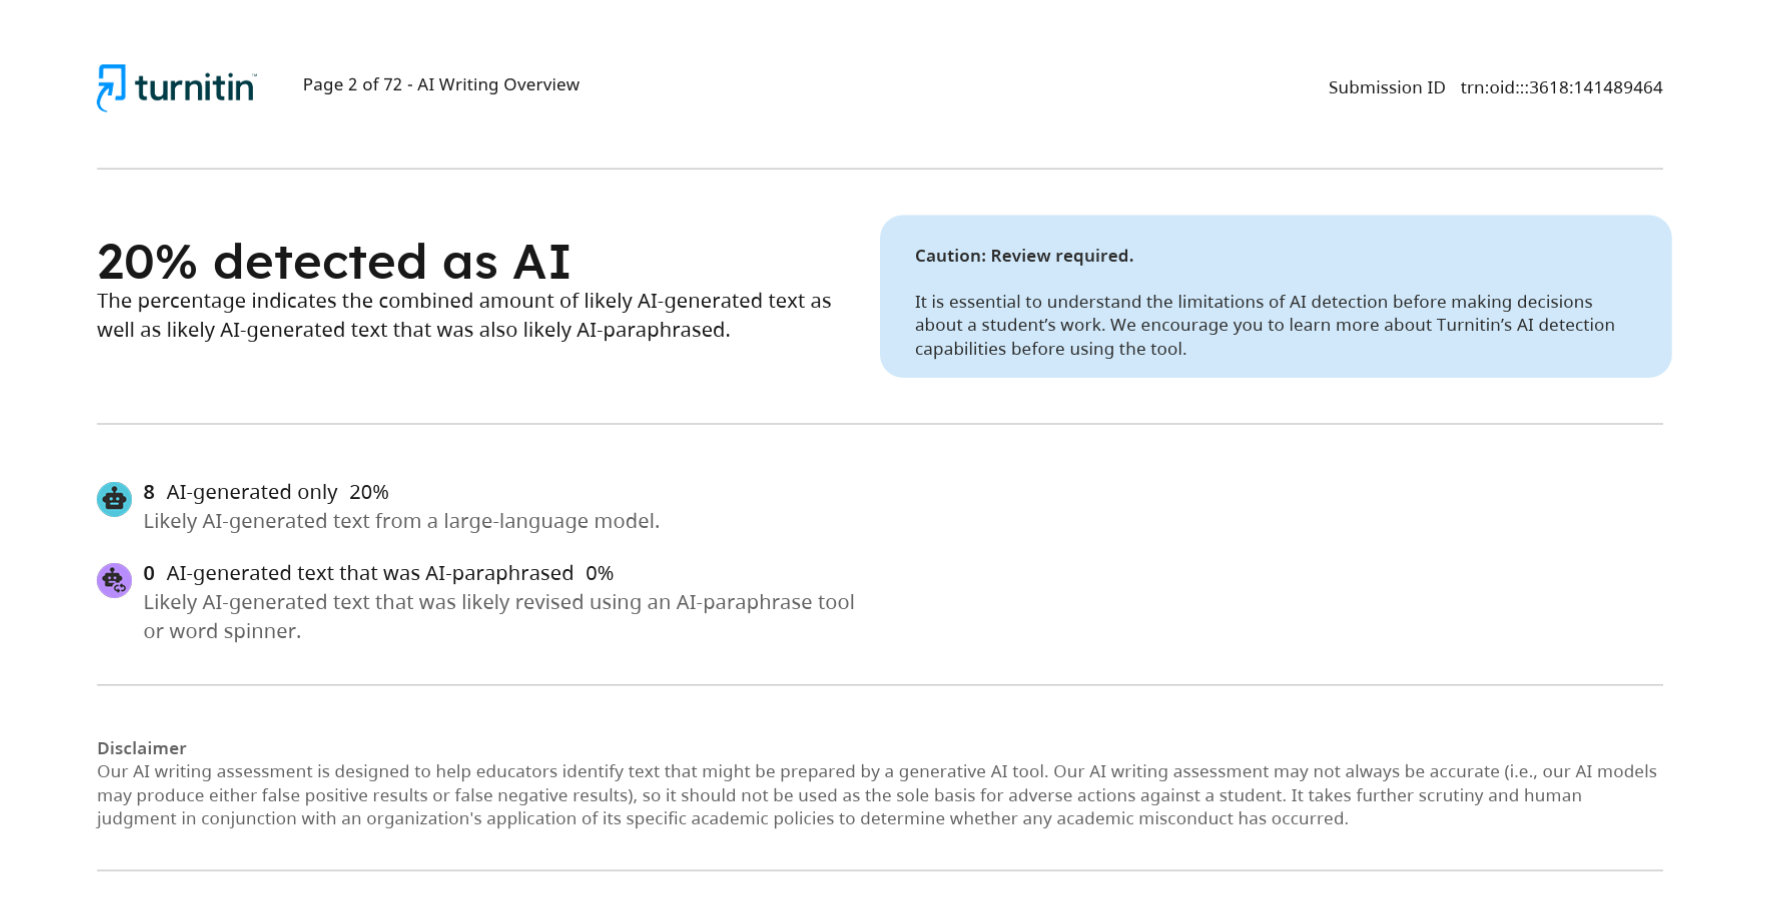
\includegraphics[width=0.95\textwidth]{Figures/plag1}
\caption[Turnitin AI writing detection overview]{\textbf{Turnitin AI writing detection overview}}
\label{fig:plag_ai}
\end{figure}

		\chapter{Publication Details}

The following paper has been submitted to \textit{IEEE Access} for peer review. The manuscript is currently under review.

\vspace{0.5cm}

\noindent\textbf{Title:} SourceSift: Detecting AI-Generated Source Code via Hybrid Syntactic-Semantic Fingerprinting Across Multiple Programming Languages

\noindent\textbf{Journal:} IEEE Access

\noindent\textbf{Manuscript ID:} Access-2026-25127

\noindent\textbf{Status:} Under Review

\noindent\textbf{Submitted:} 26-May-2026

\vspace{0.5cm}

\begin{figure}[htb]
\centering
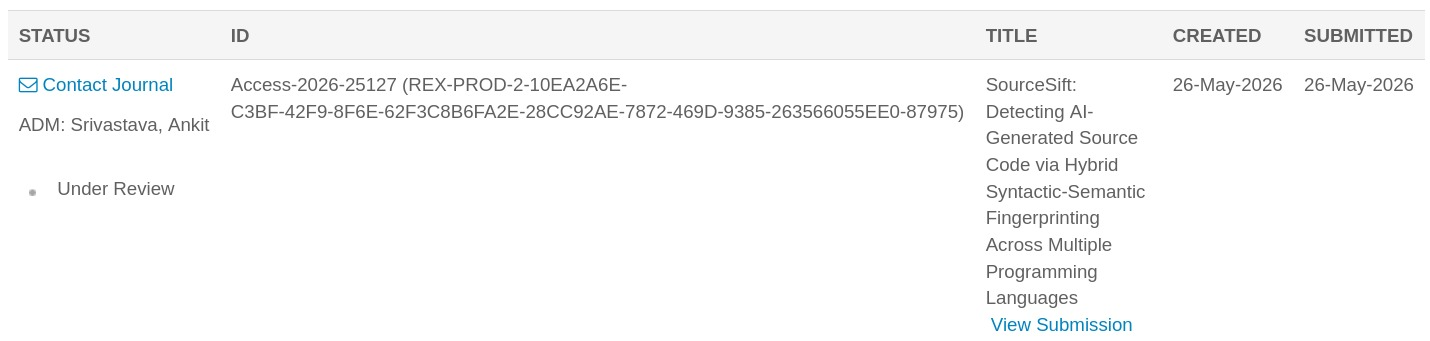
\includegraphics[width=0.95\textwidth]{Figures/Adnan_1}
\caption{IEEE Author Portal submission status}
\label{fig:pub_status}
\end{figure}

\begin{figure}[htb]
\centering

\includegraphics[width=0.95\textwidth]{Figures/Adnan_2}
\caption{Manuscript submission confirmation from IEEE Access}
\label{fig:pub_confirm}
\end{figure}

		\chapter{Algorithms}

This appendix presents the key algorithms used in Ansieyes in pseudocode form. Due to the corporate nature of the project, actual source code has been omitted in favour of algorithmic descriptions.

\section{Issue Analysis Pipeline}

\begin{tcblisting}{listing only,colback=gray!10!white, breakable, boxsep=0pt,top=1mm,bottom=1mm,left=1mm,right=1mm,
listing options={
basicstyle=\small\ttfamily,
commentstyle=\color{gray},
backgroundcolor=\color{gray!25}}}
ALGORITHM: AnalyseIssue(title, description, codebase, retries)
--------------------------------------------------------------
INPUT:  Issue title, description, codebase text, max retries
OUTPUT: Structured analysis (type, severity, root cause, solutions)

1. Load codebase content from Repomix output file
2. Build prompt = SystemRole + title + description + codebase
                  + JSON format instructions
3. FOR attempt = 0 TO retries DO
     response = CallGeminiAPI(prompt)
     json_data = ExtractJSON(response)   -- try 3 strategies
     IF json_data is valid THEN
       analysis = ParseToModel(json_data)
     ELSE
       analysis = FallbackTextExtraction(response)
     END IF
     IF IsHighQuality(analysis) THEN
       RETURN analysis
     END IF
   END FOR
4. RETURN best available analysis
\end{tcblisting}

\section{Quality Validation}

\begin{tcblisting}{listing only,colback=gray!10!white, breakable, boxsep=0pt,top=1mm,bottom=1mm,left=1mm,right=1mm,
listing options={
basicstyle=\small\ttfamily,
commentstyle=\color{gray},
backgroundcolor=\color{gray!25}}}
ALGORITHM: IsHighQuality(analysis)
----------------------------------
INPUT:  Parsed analysis object
OUTPUT: Boolean (true if acceptable quality)

IF count(analysis.solutions) < 1       THEN RETURN false
IF analysis.confidence < 0.3           THEN RETURN false
IF analysis.summary.length < 20        THEN RETURN false
IF analysis.primary_cause.length < 10  THEN RETURN false
IF any file path contains "path/to/"   THEN RETURN false
IF any file path contains "example.py" THEN RETURN false
IF any solution description < 10 chars THEN RETURN false
RETURN true
\end{tcblisting}

\section{Prompt Injection Detection}

\begin{tcblisting}{listing only,colback=gray!10!white, breakable, boxsep=0pt,top=1mm,bottom=1mm,left=1mm,right=1mm,
listing options={
basicstyle=\small\ttfamily,
commentstyle=\color{gray},
backgroundcolor=\color{gray!25}}}
ALGORITHM: DetectInjection(text)
--------------------------------
INPUT:  Issue text to evaluate
OUTPUT: Risk level, confidence, detected patterns

-- Layer 1: ML-based
ml_score = PytectorModel.classify(text)
ml_detected = (ml_score > 0.5)

-- Layer 2: Pattern matching across 7 categories
patterns_found = []
FOR each category in [role, system, bypass, file,
                      code, extraction, leakage] DO
  FOR each regex in category.patterns DO
    IF regex matches text THEN
      patterns_found.add(category)
    END IF
  END FOR
END FOR
pattern_score = lookup_confidence(patterns_found)

-- Layer 3: Heuristic analysis
heuristic_score = 0
IF special_char_sequences(text) > 3    THEN score += 0.6
IF instruction_keywords(text) > 3      THEN score += 0.7
IF suspicious_delimiters(text) > 2     THEN score += 0.5
IF max_sentence_length(text) > 100     THEN score += 0.4

-- Aggregate
final_confidence = MAX(ml_score, pattern_score,
                       heuristic_score)
pattern_count = len(unique(patterns_found))
risk = ClassifyRisk(final_confidence, pattern_count)
RETURN InjectionResult(risk, final_confidence, patterns)
\end{tcblisting}

\section{Cosine Similarity Duplicate Detection}

\begin{tcblisting}{listing only,colback=gray!10!white, breakable, boxsep=0pt,top=1mm,bottom=1mm,left=1mm,right=1mm,
listing options={
basicstyle=\small\ttfamily,
commentstyle=\color{gray},
backgroundcolor=\color{gray!25}}}
ALGORITHM: CosineDuplicateDetect(new_title, new_desc,
                                 existing_issues, threshold)
-----------------------------------------------------
INPUT:  New issue title and description,
        list of existing issues, threshold (default 0.6)
OUTPUT: Duplicate detection result

1. FOR each issue (new + existing) DO
     text = lowercase(title + " " + title + " " + desc)
     text = remove_special_chars(text)
     text = normalise_whitespace(text)
   END FOR
2. Build TF-IDF matrix using unigrams and bigrams
   (max 5000 features, English stop words removed)
3. Compute cosine similarity between new issue
   vector and all existing issue vectors
4. Find max_similarity and best_match_index
5. IF max_similarity >= threshold THEN
     confidence = MIN(max_similarity * 1.2, 1.0)
     RETURN DuplicateResult(true, existing[best_match],
                            max_similarity, confidence)
   ELSE
     RETURN DuplicateResult(false, null,
                            max_similarity, max_similarity)
   END IF
\end{tcblisting}

\section{Librarian File Selection}

\begin{tcblisting}{listing only,colback=gray!10!white, breakable, boxsep=0pt,top=1mm,bottom=1mm,left=1mm,right=1mm,
listing options={
basicstyle=\small\ttfamily,
commentstyle=\color{gray},
backgroundcolor=\color{gray!25}}}
ALGORITHM: LibrarianFileSelection(title, desc, chunks)
------------------------------------------------------
INPUT:  Issue title, description, directory chunks
OUTPUT: List of relevant file paths

1. Load all .txt files from chunks directory
2. Send directory list to Gemini:
   "Which directories are relevant to this issue?"
3. Validate returned directory names against loaded chunks
4. FOR each relevant chunk DO
     Send chunk content to Gemini:
     "Which files in this directory are relevant?"
     FOR each returned path DO
       IF path has "/" AND has extension
          AND length < 200
          AND not a comment line THEN
         Add to relevant_files set
       END IF
     END FOR
   END FOR
5. RETURN relevant_files
\end{tcblisting}

	\end{spacing}
\end{document}
